%%%%%%%%%%%%%%%%%%%%%%%%%%
% MSc Project Background Report Template
% Prof. Roger K. Moore
% University of Sheffield
% 22 March 2017
%%%%%%%%%%%%%%%%%%%%%%%%%%


\documentclass[11pt,oneside]{book}
\usepackage[margin=1.2in]{geometry}
\usepackage{setspace}
\usepackage[toc,page]{appendix}
\usepackage{graphicx}
\usepackage[hyphens]{url}
\usepackage{microtype}
\usepackage{amsmath}
\usepackage{amsfonts}
\usepackage{amssymb}
\usepackage[T1]{fontenc}
\usepackage[utf8]{inputenc}
\usepackage{booktabs}
\usepackage{multirow}
\usepackage{makecell}
\usepackage{float}

% Better line breaking and hyphenation
\tolerance=1000
\emergencystretch=5pt
\hbadness=1000

\begin{document}

\frontmatter

\begin{titlepage}

% You need to edit the details here

\begin{center}

\includegraphics[width=5cm]{images/UOSLogo_Portrait_Violet_RGB.png}\\[2cm]
\linespread{1.2}\huge {\bfseries Robustness of MEMIT Knowledge Editing in Large Language Models: A Comparative Study on LLaMA 3.1 and DeepSeek}\\[2cm]
\linespread{1}
{\Large Benjamin Tenbuuren}\\[1cm]
{\large \emph{Supervisor:} Dr. Cass Zhixue Zhao}\\[1cm]
\large \emph{A report submitted in fulfilment of the requirements}\\ \emph{for the degree of} MSc in Artificial Intelligence\\[0.3cm] 
\textit{in the}\\[0.3cm]
School of Computer Science\\[2cm]
\today
\end{center}

\end{titlepage}

% -------------------------------------------------------------------
% Declaration
% -------------------------------------------------------------------

\newpage
\chapter*{\Large Declaration}

\setstretch{1.1} % set the line spacing differently if you wish, but this looks good to me. 

All sentences or passages quoted in this report from other people's work have been specifically acknowledged by clear cross-referencing to author, work and page(s). Any illustrations that are not the work of the author of this report have been used with the explicit permission of the originator and are specifically acknowledged. I understand that failure to do this amounts to plagiarism and will be considered grounds for failure in this project and the degree examination as a whole.\\[1cm]

\noindent Name:\\[1mm]
\rule[1em]{25em}{0.5pt}

\noindent Signature:\\[1mm]
\rule[1em]{25em}{0.5pt}

\noindent Date:\\[1mm]
\rule[1em]{25em}{0.5pt}

% -------------------------------------------------------------------
% Abstract
% -------------------------------------------------------------------

\chapter*{\Large \center Abstract}

Lorem ipsum dolor sit amet, consectetuer adipiscing elit. Aenean commodo ligula eget dolor. Aenean massa. Cum sociis natoque penatibus et magnis dis parturient montes, nascetur ridiculus mus. Donec quam felis, ultricies nec, pellentesque eu, pretium quis, sem. Nulla consequat massa quis enim. Donec pede justo, fringilla vel, aliquet nec, vulputate eget, arcu. In enim justo, rhoncus ut, imperdiet a, venenatis vitae, justo. Nullam dictum felis eu pede mollis pretium. Integer tincidunt. Cras dapibus. Vivamus elementum semper nisi. Aenean vulputate eleifend tellus. Aenean leo ligula, porttitor eu, consequat vitae, eleifend ac, enim. Aliquam lorem ante, dapibus in, viverra quis, feugiat a, tellus. Phasellus viverra nulla ut metus varius laoreet. Quisque rutrum. Aenean imperdiet. Etiam ultricies nisi vel augue. Curabitur ullamcorper ultricies nisi. Nam eget dui. Etiam rhoncus. Maecenas tempus, tellus eget condimentum rhoncus, sem quam semper libero, sit amet adipiscing sem neque sed ipsum. Nam quam nunc, blandit vel, luctus pulvinar, hendrerit id, lorem. Maecenas nec odio et ante tincidunt tempus. Donec vitae sapien ut libero venenatis faucibus. Nullam quis ante. Etiam sit amet orci eget eros faucibus tincidunt. Duis leo. Sed fringilla mauris sit amet nibh. Donec sodales sagittis magna. Sed consequat, leo eget bibendum sodales, augue velit cursus nunc.


% -------------------------------------------------------------------
% TOC etc
% -------------------------------------------------------------------

\tableofcontents
\listoffigures
\listoftables

\setstretch{1.1} 

\mainmatter

\chapter{Introduction}

Large language models have achieved remarkable capabilities in natural language understanding and generation, yet they face a fundamental challenge: the factual knowledge encoded within their parameters becomes outdated over time and may contain inaccuracies from their training data. When a model incorrectly states that ``Barack Obama was born in Hawaii in 1962'' or fails to recognize recent world events, the consequences extend beyond mere technical limitations to real-world applications in healthcare, education, and critical decision-making systems \cite{brown_2020_language}. 

Traditional approaches of retraining entire models to correct such factual errors are computationally prohibitive and impractical for deployment scenarios requiring rapid knowledge updates.

The distributed nature of knowledge representation in neural networks complicates selective updates. Unlike databases where factual information can be precisely located and modified, neural knowledge exists as distributed patterns across millions of parameters within transformer feed-forward networks \cite{geva_2021_transformer, meng_2022_locating}. 

Standard fine-tuning approaches suffer from catastrophic forgetting, where learning new information degrades previously acquired knowledge \cite{mccloskey_1989_catastrophic}. The temporal mismatch between model development cycles and the rapid pace of factual changes creates a persistent knowledge gap that traditional methods cannot efficiently address.

Neural model editing represents a paradigm shift toward precise, localized modifications of model behavior through direct parameter manipulation. Unlike fine-tuning approaches that rely on gradient-based optimization over multiple training iterations, model editing techniques aim to identify and modify the specific parameters responsible for storing target factual associations \cite{mitchell_2022_mend}. 

This approach enables single-step interventions that can change model outputs for specific inputs while minimizing unintended consequences on unrelated knowledge.

Recent advances in model editing have produced two prominent algorithmic approaches: the Rank-One Model Editing (ROME) algorithm, which enables precise individual fact modifications through rank-one weight updates \cite{mitchell_2022_rome}, and the Mass-Editing Memory in a Transformer (MEMIT) algorithm, which facilitates simultaneous editing of multiple facts through batch processing \cite{meng_2022_memit}. 

Both methods leverage causal tracing analysis to identify critical layers where factual information is stored and retrieved, enabling targeted interventions in transformer feed-forward networks.

Despite these advances, significant gaps remain in understanding optimal layer selection strategies and scaling behavior across different editing volumes. Current approaches rely on heuristic layer selection methods that may not generalize across transformer architectures. 

Furthermore, the comparative advantages of MEMIT versus ROME under varying conditions remain insufficiently characterized, particularly regarding their effectiveness across different scales of simultaneous edits and their impact on downstream task performance.

This dissertation investigates neural model editing techniques that enable precise, efficient modification of factual associations while preserving model capabilities. Through systematic comparison of MEMIT and ROME algorithms across multiple transformer architectures and editing scales, this research advances the theoretical understanding and practical deployment of knowledge modification systems for large language models.

\section{Aim and Objective}
\label{sec:aim_objective}

The primary aim of this research is to advance neural model editing methodologies through comprehensive evaluation of layer selection optimization, scaling behavior characterization, and edit persistence analysis. This investigation seeks to establish principled foundations for precise, efficient knowledge modification in large language models while understanding their interaction with parameter-efficient fine-tuning approaches.

\textbf{Importantly, this research represents the first comprehensive investigation of neural model editing on DeepSeek-R1-Distill-Llama-8B—a state-of-the-art architecture that has never been studied in the context of knowledge editing.} This pioneering exploration establishes foundational knowledge for editing advanced model architectures and contributes novel empirical insights to the field.

The research addresses three specific objectives:

\textbf{Objective 1: Layer Selection Optimization.} Establish and validate optimal layer selection methodologies for neural model editing through systematic comparison of causal tracing approaches. This includes developing frozen component analysis techniques to isolate MLP and attention contributions, implementing gap-based selection strategies, and validating effectiveness across Llama-3.1-8B-Instruct and DeepSeek-R1-Distill-Llama-8B architectures to identify MLP-dominant layers most suitable for MEMIT editing.

\textbf{Objective 2: Scaling Behavior Characterization.} Investigate MEMIT's effectiveness and limitations across five orders of magnitude of simultaneous edits, from single fact modifications to mass editing of 10,000 factual associations. This analysis will identify critical scaling thresholds, characterize performance degradation patterns, and establish optimal operating regimes for different deployment scenarios, providing empirical boundaries for practical model editing applications.

\textbf{Objective 3: Edit Persistence Under Fine-tuning.} Determine whether model-edited factual knowledge persists after subsequent parameter-efficient fine-tuning operations, specifically examining the interaction between MEMIT modifications and LoRA/DoRA fine-tuning approaches. This investigation will evaluate edit retention rates, identify potential interference patterns, and establish protocols for combining knowledge editing with fine-tuning methodologies in practical deployment pipelines.

These objectives collectively address the fundamental research question: How can neural model editing be optimized to achieve reliable layer selection, scalable knowledge modification, and persistent edit retention in the context of modern parameter-efficient fine-tuning workflows?

\section{Overview of the Report}
\label{sec:report_overview}

This dissertation is structured to provide systematic investigation of neural model editing methodologies through six interconnected chapters that progress from theoretical foundations to practical applications.

\textbf{Chapter 2: Literature Review} examines the theoretical foundations of transformer knowledge storage mechanisms and surveys existing model editing approaches. This chapter positions the current research within the broader context of neural knowledge modification techniques and identifies key methodological gaps that motivate the experimental design.

\textbf{Chapter 3: Methodology} details the experimental framework including causal tracing protocols, frozen component analysis procedures, and evaluation metrics. This chapter establishes the rigorous experimental design that enables systematic comparison of editing algorithms across multiple conditions and architectures.

\textbf{Chapter 4: Results} presents comprehensive evaluation of MEMIT across different scales, layer selections, and model architectures. This chapter characterizes layer selection optimization findings, scaling behavior patterns, and provides empirical analysis of performance boundaries across five orders of magnitude of simultaneous edits.

\textbf{Chapter 5: Discussion} integrates experimental findings to address the three research objectives, analyzing layer selection methodologies, scaling behavior implications, and edit persistence under fine-tuning. This chapter synthesizes results to establish principled guidelines for neural model editing deployment and identifies the interaction patterns between knowledge editing and parameter-efficient fine-tuning approaches.

The dissertation concludes with implications for neural model editing deployment and directions for future research in knowledge modification systems. Each chapter builds systematically toward comprehensive understanding of optimal editing strategies for maintaining factual accuracy in large language models.

\chapter{Literature Review}

The rapid advancement of large language models (LLMs) has revolutionized natural language processing, demonstrating remarkable capabilities in tasks ranging from text generation to complex reasoning \cite{brown_2020_language, touvron_2023_llama}. However, the static nature of these models poses significant challenges when factual knowledge becomes outdated or requires correction. This chapter provides a comprehensive review of neural model editing techniques, with particular emphasis on the MEMIT and ROME algorithms that form the foundation of this research, alongside parameter-efficient fine-tuning methods such as LoRA and DoRA that offer complementary approaches to model adaptation.

\section{Foundations of Neural Model Editing}

\subsection{Knowledge Storage in Transformer Models}

Understanding how factual knowledge is stored and retrieved in transformer architectures is fundamental to developing effective editing techniques. Geva et al. \cite{geva_2021_transformer} provided seminal insights by proposing that transformer feed-forward layers function as key-value memories, where the first linear transformation acts as a key encoder and the second as a value retrieval mechanism. This conceptualization forms the theoretical foundation for direct weight editing approaches.

The transformer architecture, introduced by Vaswani et al. \cite{vaswani_2017_attention}, relies on multi-head attention mechanisms and position-wise feed-forward networks. Recent work has shown that factual associations are primarily stored in the middle layers of these networks, particularly within the multi-layer perceptron (MLP) components \cite{petroni_2019_language, jiang_2020_how}. This localization of factual knowledge storage has enabled targeted editing approaches that modify specific model weights without affecting the entire network.

\subsection{The Challenge of Catastrophic Forgetting}

Traditional fine-tuning approaches for updating model knowledge suffer from catastrophic forgetting, where learning new information interferes with previously acquired knowledge \cite{mccloskey_1989_catastrophic}. While techniques such as elastic weight consolidation have been proposed to mitigate this issue \cite{kirkpatrick_2017_overcoming}, they remain computationally expensive and may not be suitable for frequent knowledge updates. This limitation has motivated the development of more targeted editing approaches that can modify specific facts without extensive retraining.

% FIGURE PLACEHOLDER: Conceptual diagram showing knowledge storage in transformer layers and the catastrophic forgetting problem

\section{Direct Memory Editing Approaches}

\subsection{Early Knowledge Editing Methods}

The field of neural model editing emerged from early work on editable neural networks \cite{sinitsin_2020_editable_neural} and fact editing in language models \cite{cao_2021_editing_factual_knowledge}. These foundational approaches demonstrated the feasibility of modifying specific factual associations within pre-trained models, though they were limited in scale and often required significant computational resources.

Cao et al. \cite{cao_2021_editing_factual_knowledge} introduced one of the first systematic approaches to editing factual knowledge in language models, demonstrating that targeted modifications could be made to BERT-style models. However, their approach was limited to relatively simple factual updates and did not scale to large transformer models or multiple simultaneous edits.

\subsection{ROME: Rank-One Model Editing}

ROME (Rank-One Model Editing), introduced by Meng et al. \cite{meng_2022_locating}, represents a significant advancement in direct model editing techniques. The algorithm operates on the principle that factual associations can be modified through rank-one updates to specific feed-forward layers within transformer models.

\subsubsection{Rank-One Weight Updates}

ROME modifies the feed-forward weights using a rank-one update. For a target layer with weight matrix $\mathbf{W}$, the update takes the form:

\begin{equation}
\mathbf{W}_{new} = \mathbf{W}_{old} + \mathbf{u}\mathbf{v}^T
\end{equation}

where $\mathbf{u}$ and $\mathbf{v}$ are vectors chosen to ensure that the new association $(k^*, v^*)$ is correctly encoded while preserving existing associations. The optimization problem seeks to minimize:

\begin{equation}
\|\mathbf{W}_{new}\mathbf{K} - \mathbf{V}\|_F^2
\end{equation}

subject to the constraint that $\mathbf{W}_{new}\mathbf{k}^* = \mathbf{v}^*$, where $\mathbf{K}$ and $\mathbf{V}$ represent existing key-value associations.

\subsubsection{Evaluation and Limitations}

ROME demonstrates effectiveness on the zsRE (zero-shot Relation Extraction) benchmark, successfully editing individual facts while maintaining model performance on unrelated tasks. However, the algorithm faces several limitations:

\begin{itemize}
    \item \textbf{Sequential editing degradation}: Performance degrades significantly when applying multiple sequential edits
    \item \textbf{Scale limitations}: The rank-one constraint limits the complexity of edits that can be performed
    \item \textbf{Layer selection}: The method requires careful selection of target layers, which may vary across model architectures
\end{itemize}

\subsection{MEMIT: Mass-Editing Memory in a Transformer}

MEMIT (Mass-Editing Memory in a Transformer), developed by \cite{meng_2022_memit}, addresses the scalability limitations of ROME by enabling simultaneous editing of thousands of factual associations. This represents a significant advancement in neural model editing, scaling beyond previous methods by orders of magnitude.

\begin{figure}[H]
\centering
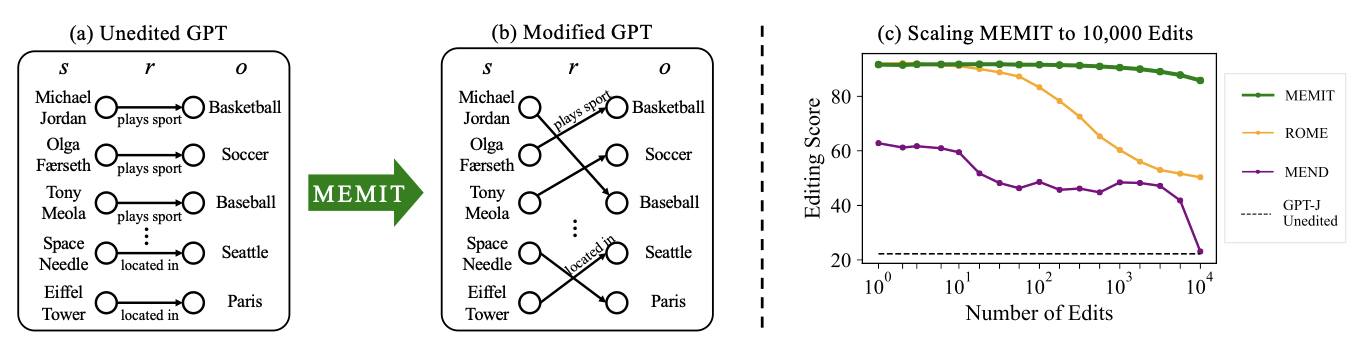
\includegraphics[width=0.85\textwidth]{figures/MEMIT_fig1.png}
\caption{MEMIT overview: (a) Language models store factual associations as (subject, relation, object) tuples, (b) MEMIT modifies these associations through targeted weight updates, and (c) performance comparison showing MEMIT's superior scaling capabilities, maintaining effectiveness up to 10,000 simultaneous edits compared to ROME and MEND methods.}
\label{fig:memit_overview}
\end{figure}

\subsubsection{Algorithmic Foundation}

Unlike ROME's single-fact editing approach, MEMIT formulates the editing problem as a batch optimization targeting multiple MLP layers simultaneously. The algorithm identifies critical layers where factual knowledge is stored and computes coordinated updates across these layers.

\begin{figure}[H]
\centering
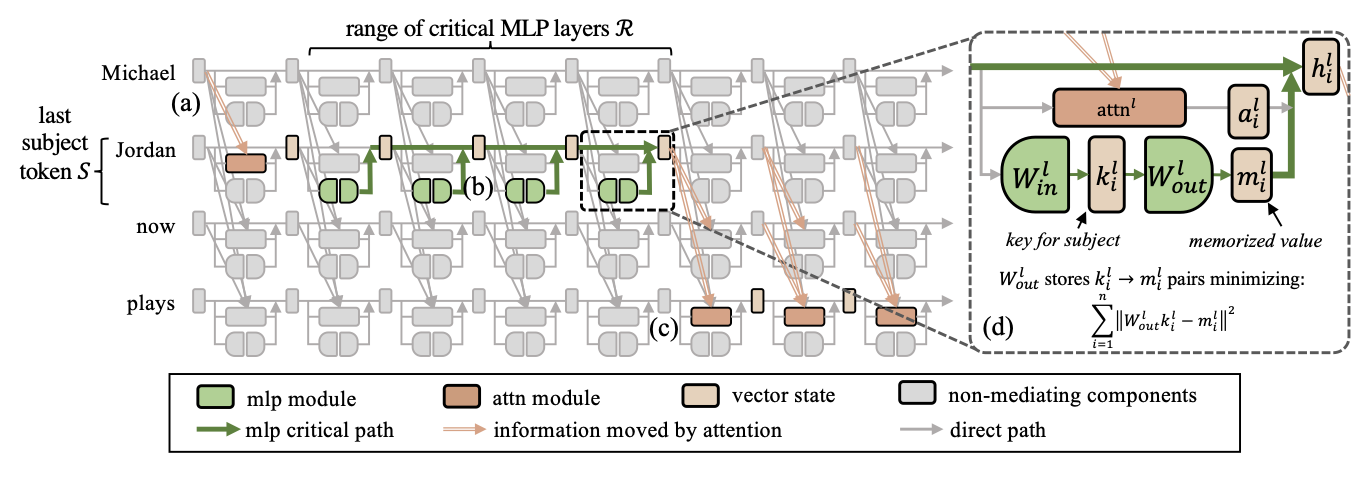
\includegraphics[width=0.95\textwidth]{figures/MEMIT_fig2.png}
\caption{MEMIT technical implementation showing the identification of critical MLP layers ($\mathcal{R}$) and the information flow during factual recall. The algorithm processes key-value pairs through multiple layers, with attention mechanisms (orange paths) and MLP modules (green paths) working together to store and retrieve factual associations.}
\label{fig:memit_technical}
\end{figure}

The multi-fact editing framework formulates the problem as a batch optimization:

\begin{equation}
\min_{\Delta\mathbf{W}} \|\mathbf{K}^T(\mathbf{W} + \Delta\mathbf{W}) - \mathbf{V}^T\|_F^2 + \lambda\|\Delta\mathbf{W}\|_F^2
\end{equation}

where $\mathbf{K}$ and $\mathbf{V}$ contain multiple key-value pairs to be edited simultaneously, and $\lambda$ controls the regularization strength to prevent overfitting.

\subsubsection{Covariance-Based Updates}

MEMIT employs a sophisticated approach based on estimating the covariance structure of the activations. The algorithm computes:

\begin{equation}
\mathbf{C} = \frac{1}{N}\sum_{i=1}^{N}\mathbf{k}_i\mathbf{k}_i^T
\end{equation}

where $\mathbf{k}_i$ represents the key vectors for the facts to be edited. This covariance matrix enables more stable updates when editing large numbers of facts simultaneously.

\subsubsection{Scaling and Performance}

MEMIT demonstrates remarkable scaling capabilities, successfully editing up to 10,000 facts simultaneously in GPT-J (6B parameters) and GPT-NeoX (20B parameters). The algorithm maintains three key properties:

\begin{enumerate}
    \item \textbf{Specificity}: Edits affect only the targeted facts without influencing unrelated knowledge
    \item \textbf{Generalization}: Edited facts generalize to paraphrases and related expressions
    \item \textbf{Fluency}: The model maintains natural language generation capabilities after editing
\end{enumerate}

Experimental results show that MEMIT achieves success rates exceeding 80\% on both the CounterFact and zsRE datasets when editing thousands of facts, significantly outperforming sequential application of ROME or other single-fact editing methods.

\section{Causal Tracing Methodology}

Causal tracing represents a fundamental technique for understanding information flow in transformer models and identifying the computational components responsible for specific behaviors. This methodology has become essential for both ROME and MEMIT algorithms in determining optimal target layers for knowledge editing.

\subsection{Theoretical Foundation}

The foundation of causal tracing lies in causal mediation analysis, which systematically identifies the causal role of intermediate representations in producing model outputs. The technique operates by:

\begin{enumerate}
    \item Running the model on a factual statement while introducing noise to disrupt normal processing
    \item Systematically restoring individual hidden states to identify which components are critical for fact retrieval
    \item Localizing the decisive computations to specific MLP modules in middle layers
\end{enumerate}

Mathematically, the causal effect of a hidden state $\mathbf{h}^{(l)}_i$ at layer $l$ and position $i$ is measured by comparing the model's output when this state is restored versus when it remains corrupted:

\begin{equation}
\mathcal{E}^{(l)}_i = \mathbb{E}[P(\text{fact} | \text{clean}_{<i}, \mathbf{h}^{(l)}_i, \text{corrupted}_{>i})] - \mathbb{E}[P(\text{fact} | \text{corrupted})]
\end{equation}

where $\mathcal{E}^{(l)}_i$ represents the causal effect of restoring the hidden state at layer $l$ and position $i$.

Both ROME and MEMIT leverage causal tracing to identify optimal target layers for knowledge editing. The technique reveals that factual knowledge is predominantly stored in middle layers of transformer models, with specific layer ranges varying across architectures. This localization enables targeted editing approaches that modify specific components while preserving overall model functionality.

% FIGURE PLACEHOLDER: Causal tracing visualization showing effect patterns across transformer layers

\section{Parameter-Efficient Fine-Tuning Methods}

While direct editing approaches like ROME and MEMIT offer precise control over factual associations, parameter-efficient fine-tuning (PEFT) methods provide complementary approaches for model adaptation. These techniques reduce the computational cost of fine-tuning while maintaining competitive performance.

\subsection{Adapter-Based Methods}

Early parameter-efficient approaches focused on introducing small adapter modules between transformer layers \cite{houlsby_2019_adapters}. These adapters contain significantly fewer parameters than full fine-tuning but can effectively adapt pre-trained models to downstream tasks. While not specifically designed for factual editing, adapters provide a foundation for understanding parameter-efficient model modification.

Prefix-tuning \cite{li_2021_prefix_tuning} and prompt-tuning \cite{lester_2021_prompt_tuning} represent alternative approaches that modify the input representation rather than the model weights. These methods demonstrate that effective adaptation can be achieved through careful manipulation of the input space, though they may be less suitable for precise factual editing tasks.

\subsection{LoRA: Low-Rank Adaptation}

LoRA (Low-Rank Adaptation), introduced by \cite{hu_2022_lora}, revolutionized parameter-efficient fine-tuning by decomposing weight updates into low-rank matrices. The core insight is that the weight changes during adaptation have low intrinsic rank.

\subsubsection{Mathematical Foundation}

For a pre-trained weight matrix $\mathbf{W}_0 \in \mathbb{R}^{d \times k}$, LoRA constrains the update $\Delta\mathbf{W}$ to be low-rank:

\begin{equation}
\mathbf{W} = \mathbf{W}_0 + \Delta\mathbf{W} = \mathbf{W}_0 + \mathbf{B}\mathbf{A}
\end{equation}

where $\mathbf{B} \in \mathbb{R}^{d \times r}$, $\mathbf{A} \in \mathbb{R}^{r \times k}$, and $r \ll \min(d,k)$ is the rank. During training, $\mathbf{W}_0$ is frozen and only $\mathbf{A}$ and $\mathbf{B}$ are updated.

\begin{figure}[H]
\centering
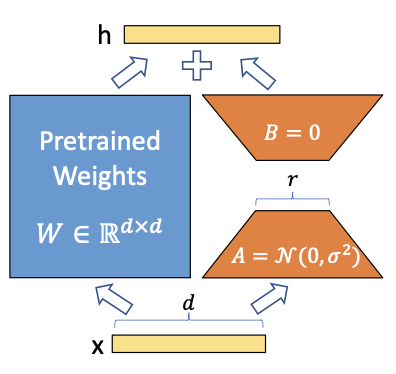
\includegraphics[width=0.5\textwidth]{figures/LoRA.png}
\caption{LoRA architecture showing the decomposition of weight updates into low-rank matrices. The original pre-trained weights $\mathbf{W}_0$ remain frozen while trainable low-rank matrices $\mathbf{A}$ and $\mathbf{B}$ capture the adaptation-specific changes.}
\label{fig:lora_architecture}
\end{figure}

\subsubsection{Efficiency and Performance}

LoRA achieves remarkable efficiency gains:
\begin{itemize}
    \item Reduces trainable parameters by up to 10,000$\times$ compared to full fine-tuning
    \item Decreases GPU memory requirements by 3$\times$
    \item Maintains or improves performance on downstream tasks
    \item Enables efficient switching between different task-specific adaptations
\end{itemize}

The method has been successfully applied to various transformer architectures, including GPT-3, where it achieves performance comparable to full fine-tuning while training only 0.01\% of the parameters.

\subsection{DoRA: Weight-Decomposed Low-Rank Adaptation}

DoRA (Weight-Decomposed Low-Rank Adaptation) \cite{liu_2024_dora} represents a recent advancement that addresses fundamental limitations in LoRA by decomposing weights into separate magnitude and direction components. This decomposition enables more nuanced parameter updates that better align with the patterns observed in full fine-tuning.

\subsubsection{Theoretical Foundation}

DoRA is motivated by empirical analysis showing that full fine-tuning and LoRA exhibit different patterns in terms of weight magnitude and direction changes. While LoRA only modifies the overall weight through additive low-rank updates, DoRA provides independent control over these two critical aspects of weight adaptation.

The method decomposes the pre-trained weight matrix as:

\begin{equation}
\mathbf{W}_0 = \mathbf{m} \frac{\mathbf{V}}{\|\mathbf{V}\|_c}
\end{equation}

where $\mathbf{m} = \|\mathbf{W}_0\|_c$ represents the magnitude component and $\frac{\mathbf{V}}{\|\mathbf{V}\|_c}$ represents the unit directional component. During adaptation, DoRA applies LoRA-style low-rank updates to the directional component while making the magnitude independently trainable:

\begin{equation}
\mathbf{W}' = \mathbf{m}' \frac{\mathbf{V} + \Delta\mathbf{V}}{\|\mathbf{V} + \Delta\mathbf{V}\|_c}
\end{equation}

where $\Delta\mathbf{V} = \mathbf{B}\mathbf{A}$ follows the standard LoRA decomposition and $\mathbf{m}'$ is the trainable magnitude parameter.

\begin{figure}[H]
\centering
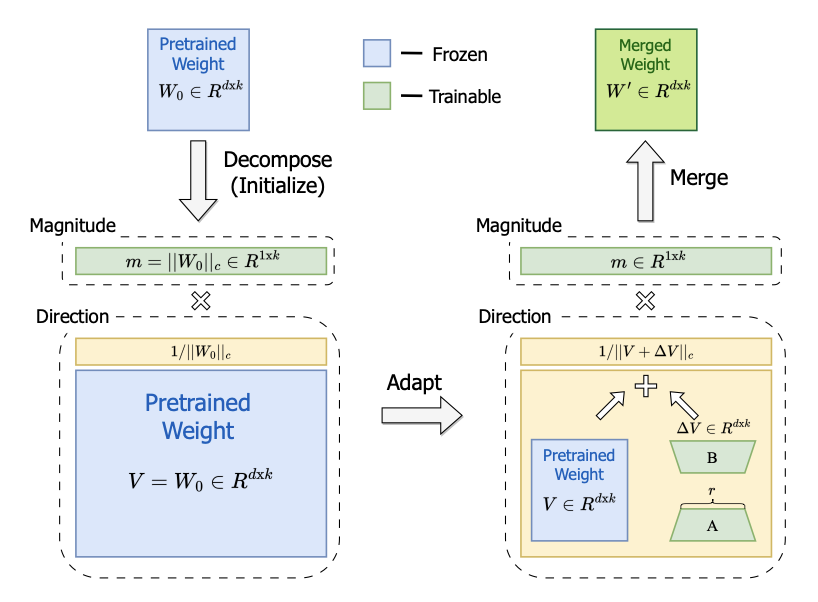
\includegraphics[width=0.7\textwidth]{figures/DoRA.png}
\caption{DoRA architecture showing the decomposition of pretrained weights into magnitude and direction components. The magnitude becomes independently trainable while the direction is updated using LoRA-style low-rank adaptation, providing more flexible parameter updates than standard LoRA.}
\label{fig:dora_architecture}
\end{figure}

\subsubsection{Advantages Over LoRA}

DoRA consistently outperforms LoRA across various tasks by addressing key limitations:

\begin{itemize}
    \item \textbf{Enhanced representational capacity}: Independent magnitude and direction control enables more flexible weight updates
    \item \textbf{Better fine-tuning alignment}: Weight update patterns more closely match those observed in full fine-tuning
    \item \textbf{Improved task performance}: Superior results on commonsense reasoning, visual instruction tuning, and multimodal understanding
    \item \textbf{Maintained efficiency}: Parameter count remains comparable to LoRA while providing enhanced learning capacity
\end{itemize}

The key insight is that magnitude and direction changes serve different roles in adaptation, and treating them independently allows for more effective parameter-efficient fine-tuning that bridges the gap between LoRA and full fine-tuning approaches.

\section{Evaluation Frameworks and Benchmarks}

\subsection{Knowledge Editing Benchmarks}

The evaluation of knowledge editing methods relies on established benchmarks that test different aspects of factual knowledge modification. Two primary datasets serve as the foundation for most knowledge editing research, each with distinct evaluation matrices and objectives.

\subsubsection{CounterFact Dataset}

The CounterFact dataset serves as a comprehensive benchmark for evaluating counterfactual knowledge editing. Each example consists of a factual statement and its counterfactual counterpart, enabling systematic evaluation of editing precision and generalization capabilities.

\textbf{Evaluation Matrix Structure:}
CounterFact employs a structured evaluation framework focusing on:
\begin{itemize}
    \item \textbf{Rewrite Success Rate}: Direct measurement of successful factual updates
    \item \textbf{Paraphrase Accuracy}: Generalization to rephrased versions of the target fact
    \item \textbf{Neighborhood Preservation}: Maintenance of related but unedited factual knowledge
    \item \textbf{Fluency Preservation}: Overall language generation quality post-editing
\end{itemize}

The dataset's strength lies in its controlled counterfactual structure, which allows for precise measurement of editing effects while minimizing confounding variables.

\subsubsection{zsRE: Zero-shot Relation Extraction}

The zsRE (Zero-shot Relation Extraction) benchmark \cite{petroni_2019_language} focuses on relational knowledge extraction and modification. Unlike CounterFact's counterfactual approach, zsRE tests the model's ability to extract and edit relational knowledge patterns without explicit training on the target relations.

\textbf{Evaluation Matrix Structure:}
zsRE employs a different evaluation framework emphasizing:
\begin{itemize}
    \item \textbf{Relation Extraction Accuracy}: Success in identifying and modifying relational patterns
    \item \textbf{Cross-relation Generalization}: Ability to generalize edits across similar relation types
    \item \textbf{Template Robustness}: Performance across different query templates and formats
    \item \textbf{Consistency Maintenance}: Preservation of logical consistency in related relations
\end{itemize}

The fundamental difference between zsRE and CounterFact lies in zsRE's focus on relational structures rather than individual factual statements, requiring more sophisticated handling of knowledge interdependencies.


\subsection{Evaluation Metrics}

Knowledge editing evaluation typically focuses on three key criteria:

\begin{enumerate}
    \item \textbf{Rewrite Success}: Whether the model correctly produces the new factual association
    \item \textbf{Paraphrase Generalization}: Whether the edit generalizes to paraphrases of the original fact
    \item \textbf{Neighborhood Preservation}: Whether related but unedited facts remain unchanged
\end{enumerate}

Additional metrics include fluency preservation, measured through perplexity on held-out text, and downstream task performance to ensure that editing does not degrade general capabilities.

\subsection{Ripple Effects and Unintended Consequences}

Recent research has highlighted the importance of evaluating ripple effects of knowledge editing \cite{wang_2023_ripple_effects}. When a fact is edited, it may have unintended consequences on related facts or reasoning chains. For example, changing "The president of the USA is Biden" might affect other facts about American politics or government structure.

The evaluation of ripple effects requires careful consideration of:
\begin{itemize}
    \item Semantic similarity between edited and potentially affected facts
    \item Logical consistency in multi-fact scenarios
    \item Long-term stability of edits over multiple inference steps
\end{itemize}

% FIGURE PLACEHOLDER: Evaluation framework diagram showing the three main criteria and their relationships

\section{Challenges and Limitations}

\subsection{Scalability Constraints}

Despite advances in methods like MEMIT, scalability remains a significant challenge:
\begin{itemize}
    \item Memory requirements grow quadratically with the number of edits
    \item Computational complexity increases substantially for large-scale editing
    \item Model-specific layer selection requires manual tuning
\end{itemize}

\subsection{Cross-Model Generalization}

Most editing methods are developed and evaluated on specific model architectures. Transfer to different architectures (e.g., from GPT to LLaMA) often requires significant adaptation, limiting the generalizability of existing approaches.

\subsection{Evaluation Gaps}

Current evaluation frameworks have several limitations:
\begin{itemize}
    \item Limited coverage of complex reasoning scenarios
    \item Insufficient evaluation of long-term stability
    \item Lack of standardized protocols for ripple effect assessment
\end{itemize}

\subsection{Integration Challenges}

The relationship between direct editing methods and parameter-efficient fine-tuning remains underexplored. Developing unified frameworks that leverage both approaches presents significant technical challenges in terms of optimization dynamics and knowledge preservation.

\section{Summary and Research Gaps}

This literature review has examined the current state of neural model editing, with particular focus on MEMIT and ROME algorithms, alongside parameter-efficient fine-tuning methods such as LoRA and DoRA. The field has made significant progress in developing methods for targeted fact editing and efficient model adaptation.

Key achievements include:
\begin{itemize}
    \item Development of scalable editing methods (MEMIT) capable of handling thousands of simultaneous edits
    \item Precise localization techniques (causal tracing) for identifying critical model components
    \item Highly efficient adaptation methods (LoRA, DoRA) that maintain performance while drastically reducing computational requirements
    \item Comprehensive evaluation frameworks for assessing editing quality and side effects
\end{itemize}

However, several research gaps remain:

\subsubsection{Layer Selection Optimization}
Current methods rely on heuristic or model-specific approaches for selecting target layers. A systematic methodology for optimal layer selection across different architectures represents a significant opportunity for improvement.

\subsubsection{Multi-Scale Editing Analysis}
While MEMIT demonstrates large-scale editing capabilities, comprehensive analysis of editing effectiveness across different scales (from single facts to tens of thousands) remains limited. Understanding the scaling behavior is crucial for practical applications.

\subsubsection{Integration of Editing and Fine-tuning}
The relationship between direct editing methods and parameter-efficient fine-tuning is underexplored. Developing unified frameworks that leverage both approaches could provide significant advantages.

\subsubsection{Cross-Architecture Generalization}
Most existing work focuses on specific model families. Developing editing methods that generalize across different transformer architectures (e.g., decoder-only vs. encoder-decoder models) remains an open challenge.

\subsubsection{Unexplored Model Architectures}
A critical gap exists in the exploration of neural model editing on recently developed architectures. The LLaMA model family, particularly \textbf{meta-llama/Llama-3.1-8B-Instruct}, represents a significant advancement in open-source language modeling. This model builds upon the foundational LLaMA architecture with substantial improvements in instruction following capabilities and multilingual performance \cite{dubey_2024_llama3}. The model employs a decoder-only transformer architecture with optimized attention mechanisms and has been fine-tuned specifically for instruction-following tasks, making it an ideal candidate for knowledge editing research due to its factual knowledge retention and generalization capabilities.

Similarly, \textbf{DeepSeek-R1-Distill-Llama-8B represents an entirely novel target for knowledge editing research—no prior work has investigated editing capabilities on this architecture}. This distilled model combines the architectural benefits of the LLaMA foundation with specialized knowledge distillation techniques, potentially offering different knowledge storage patterns that could affect editing effectiveness. The comparative study of these two architectures provides unprecedented insights into how different training methodologies and architectural optimizations influence knowledge editing performance.

This dissertation addresses several of these gaps by developing novel layer selection methodologies based on causal tracing analysis, conducting comprehensive multi-scale evaluation across different model architectures, and investigating the integration of editing techniques with parameter-efficient fine-tuning approaches. \textbf{Crucially, this work presents the first comprehensive study of neural model editing on DeepSeek-R1-Distill-Llama-8B, establishing foundational knowledge for editing this advanced architecture.} The following chapters detail the methodology and experimental results that advance the state of knowledge in neural model editing.
\chapter{Methodology}

This chapter presents the experimental methodology employed to investigate neural model editing techniques for factual knowledge modification in large language models. The research focuses on systematic evaluation of the MEMIT (Mass-Editing Memory in a Transformer) algorithm across multiple layer selection strategies, model architectures, and editing scales. The methodology encompasses novel causal tracing approaches for layer selection, comprehensive multi-scale editing evaluation, and post-editing fine-tuning analysis to assess the preservation of model capabilities.

\section{Research Questions and Hypotheses}

The research investigates three primary questions concerning neural model editing effectiveness:

\textbf{Research Question 1:} How do different layer selection methodologies, including novel causal tracing with frozen components, influence the effectiveness of knowledge editing in transformer models?

\textit{Hypothesis 1:} Layer selection strategies that incorporate component-specific causal analysis (frozen MLP/attention) will demonstrate superior editing performance compared to traditional approaches, as the frozen component analysis isolates the contribution of specific architectural elements to factual knowledge storage.

\textbf{Research Question 2:} How does the MEMIT algorithm scale across different magnitudes of simultaneous fact modifications, and what are the implications for practical deployment of neural model editing?

\textit{Hypothesis 2:} MEMIT performance will degrade as the number of simultaneous edits increases from single facts to massive scales (10,000 edits), with optimal performance occurring at intermediate scales (100-1,000 edits) where batch processing benefits outweigh interference effects.

\textbf{Research Question 3:} How do architectural differences between Llama-3.1-8B-Instruct and DeepSeek-R1-Distill-Llama-8B affect neural model editing effectiveness, particularly for DeepSeek's first evaluation in the model editing context?

\textit{Hypothesis 3:} The distillation process in DeepSeek-R1-Distill-Llama-8B will result in distinct optimal layer configurations compared to Llama-3.1-8B-Instruct, requiring adapted layer selection strategies despite shared architectural foundations.

\section{Model Selection and Rationale}

\subsection{Primary Model Architectures}

Two transformer architectures were selected for comprehensive evaluation based on their shared architectural foundation and distinct training paradigms:

\textbf{Llama-3.1-8B-Instruct} serves as the primary experimental model due to its:
\begin{itemize}
    \item Established performance in neural model editing literature
    \item Balanced parameter count (8B) enabling comprehensive experimentation
    \item Instruction-tuned capabilities facilitating robust downstream evaluation
    \item Well-documented architectural specifications for causal analysis
\end{itemize}

\textbf{DeepSeek-R1-Distill-Llama-8B} was selected as the comparative architecture to:
\begin{itemize}
    \item Provide the first systematic evaluation of DeepSeek models in neural editing context
    \item Assess the impact of knowledge distillation on editing effectiveness
    \item Evaluate cross-architectural generalization despite shared Llama foundations
    \item Maintain parameter count consistency for controlled comparison
\end{itemize}

The selection of these architectures enables investigation of how different training paradigms (instruction tuning vs. distillation) affect the localization and editability of factual knowledge within transformer models.

\subsection{Experimental Sequence}

The experimental design follows a systematic progression:
\begin{enumerate}
    \item \textbf{Primary Analysis}: Comprehensive evaluation on Llama-3.1-8B-Instruct across all layer selection methods and editing scales
    \item \textbf{Comparative Analysis}: Application of optimal methodologies to DeepSeek-R1-Distill-Llama-8B
    \item \textbf{Cross-Model Validation}: Assessment of layer selection strategy transferability between architectures
\end{enumerate}

\section{Layer Selection Methodologies}

The research employs four distinct layer selection approaches to identify optimal editing targets, each representing different theoretical foundations for factual knowledge localization in transformer models.

\subsection{Method 1: Causal Tracing with Frozen MLP Components}

This novel approach extends traditional causal tracing by selectively freezing MLP components during intervention analysis. The methodology isolates attention mechanism contributions to factual knowledge processing:

\textbf{Protocol:}
\begin{enumerate}
    \item Freeze all MLP modules across target layers: $\text{FFN}^{(l)}(\mathbf{h}) = \text{FFN}_{\text{frozen}}^{(l)}(\mathbf{h})$
    \item Apply noise corruption exclusively to attention mechanisms
    \item Compute layer-wise causal effects with isolated attention contribution:
    \begin{equation}
    \mathcal{E}_{\text{frozen-MLP}}^{(l)} = \mathbb{E}_{x \sim \mathcal{D}} \left[ \| \mathbf{h}_{\text{clean}}^{(l)}(x) - \mathbf{h}_{\text{corrupted-attn}}^{(l)}(x) \|_2 \right]
    \end{equation}
\end{enumerate}

\textbf{Layer Selection Criteria:}
Layer selection employs a gap-based threshold approach:
\begin{itemize}
    \item Identify peak causal effect layer: $l_{\text{peak}} = \text{argmax}_l \mathcal{E}_{\text{frozen-MLP}}^{(l)}$
    \item Calculate gap threshold: $\tau = 0.8 \times \max_l \mathcal{E}_{\text{frozen-MLP}}^{(l)}$
    \item Select layers where: $\mathcal{E}_{\text{frozen-MLP}}^{(l)} \geq \tau$
\end{itemize}

\textbf{Results:} Application of this methodology yielded:
\begin{itemize}
    \item \textbf{Llama-3.1-8B-Instruct}: Layers 1-6 (6 layers)
    \item \textbf{DeepSeek-R1-Distill-Llama-8B}: Layers 1-5 (5 layers)
\end{itemize}

\subsection{Method 2: Top-5 Standard Causal Tracing}

Traditional causal tracing identifies layers with highest factual knowledge sensitivity through standard intervention analysis:

\textbf{Causal Effect Computation:}
\begin{equation}
\mathcal{E}^{(l)} = \mathbb{E}_{x \sim \mathcal{D}} \left[ \| \mathbf{h}_{\text{clean}}^{(l)}(x) - \mathbf{h}_{\text{corrupted}}^{(l)}(x) \|_2 \right]
\end{equation}

\textbf{Layer Selection:}
Select the top 5 layers by causal effect magnitude:
\begin{equation}
\mathcal{L}_{\text{top-5}} = \{\text{top-5 layers by } \mathcal{E}^{(l)}\}
\end{equation}

\textbf{Results:}
\begin{itemize}
    \item \textbf{Llama-3.1-8B-Instruct}: Layers 3-7
    \item \textbf{DeepSeek-R1-Distill-Llama-8B}: Layers 2-6
\end{itemize}

\subsection{Method 3: Llama-2 EasyEdit Literature Layers}

This approach leverages established layer selections from the neural model editing literature, specifically the EasyEdit framework's optimized layers for Llama-2 architectures:

\textbf{Rationale:} The EasyEdit library has empirically determined optimal editing layers for Llama-2 through extensive experimentation. Given the architectural similarities between Llama-2 and the target models, these layers provide a literature-validated baseline.

\textbf{Layer Configuration:}
\begin{itemize}
    \item \textbf{Both Models}: Layers 4-8 (5 consecutive layers)
    \item \textbf{Theoretical Basis}: Mid-layer positioning balances feature representation and output generation phases
\end{itemize}

\subsection{Method 4: GPT2-XL MEMIT Paper Layers}

This methodology applies the original MEMIT paper's layer selection for GPT2-XL, providing insight into cross-architectural transferability:

\textbf{Historical Context:} The original MEMIT algorithm was validated on GPT2-XL using layers 13-17, representing the model's output generation layers where factual knowledge is transformed into linguistic output.

\textbf{Layer Mapping:} Direct application without architectural scaling:
\begin{itemize}
    \item \textbf{Both Models}: Layers 13-17 (5 consecutive layers)
    \item \textbf{Architectural Position}: Late-layer editing targeting output generation mechanisms
\end{itemize}

\section{MEMIT Algorithm Implementation}

\subsection{Core MEMIT Methodology}

MEMIT enables simultaneous modification of multiple facts through matrix-based parameter updates. The algorithm computes optimal weight modifications by solving:

\begin{equation}
\mathbf{W}^{(l)}_{\text{new}} = \mathbf{W}^{(l)} + \mathbf{U} \mathbf{V}^T
\end{equation}

where the update matrices are derived through:

\textbf{Key Vector Extraction:}
For each fact $i$ to be edited, extract the key representation:
\begin{equation}
\mathbf{k}_i = \text{MLP}^{(l)}(\mathbf{h}_i^{(l-1)})
\end{equation}

\textbf{Covariance Matrix Computation:}
\begin{equation}
\mathbf{C} = \frac{1}{N} \sum_{i=1}^{N} \mathbf{k}_i \mathbf{k}_i^T + \lambda \mathbf{I}
\end{equation}

where $\lambda$ provides numerical stabilization and $N$ represents the number of facts being edited simultaneously.

\textbf{Update Matrix Derivation:}
\begin{equation}
\mathbf{U} = \mathbf{C}^{-1} \mathbf{K}, \quad \mathbf{V} = \Delta \mathbf{V}_{\text{target}}
\end{equation}

where $\mathbf{K} = [\mathbf{k}_1, \mathbf{k}_2, \ldots, \mathbf{k}_N]$ contains all key vectors and $\Delta \mathbf{V}_{\text{target}}$ represents the desired output changes.

\subsection{Multi-Scale Editing Framework}

The research evaluates MEMIT performance across five orders of magnitude to assess scalability:

\begin{itemize}
    \item \textbf{Single Edit (N=1):} Individual fact modification precision
    \item \textbf{Small Batch (N=10):} Limited interference assessment  
    \item \textbf{Medium Scale (N=100):} Practical editing scenario evaluation
    \item \textbf{Large Scale (N=1000):} High-volume editing capability
    \item \textbf{Massive Scale (N=10000):} Algorithm limitation exploration
\end{itemize}

For each scale $N$, the success rate is quantified as:
\begin{equation}
\text{Success Rate}(N) = \frac{\sum_{i=1}^{N} \mathbb{1}[\text{edit}_i \text{ successful}]}{N}
\end{equation}

\subsection{Hyperparameter Configuration}

MEMIT parameters were optimized through preliminary experiments and maintained consistently across all conditions:

\begin{itemize}
    \item Learning rate: $v\_lr = 5 \times 10^{-1}$
    \item Gradient steps: $v\_num\_grad\_steps = 25$
    \item KL divergence factor: $kl\_factor = 0.0625$
    \item Momentum adjustment: $mom2\_adjustment = \text{True}$
    \item Weight decay: $v\_weight\_decay = 1 \times 10^{-3}$
    \item Context template: $[5, 10]$ and $[10, 10]$ tokens
    \item Momentum samples: $mom2\_n\_samples = 1000$
\end{itemize}

\section{Datasets and Evaluation Framework}

\subsection{Primary Evaluation Datasets}

\textbf{CounterFact Dataset (MCF)} serves as the primary factual editing benchmark:
\begin{itemize}
    \item 21,919 factual statements with counterfactual alternatives
    \item Structured format: (subject, relation, old\_object, new\_object)
    \item Example: ("Eiffel Tower", "located in", "Paris", "Rome")
    \item Comprehensive entity relationship coverage
\end{itemize}

\textbf{Zero-shot Relation Extraction Dataset (zsRE)} provides complementary assessment:
\begin{itemize}
    \item 24,543 relation extraction instances
    \item Template-based evaluation for consistency
    \item Assessment of generalization beyond direct fact memorization
    \item Focus on reasoning capability preservation
\end{itemize}

\subsection{Dataset-Specific Evaluation Metrics}

The evaluation framework employs dataset-specific metrics to capture different aspects of editing quality:

\subsubsection{zsRE Dataset Metrics}

\textbf{Rewrite Accuracy ($\text{Acc}_{\text{rewrite}}$):}
\begin{equation}
\text{Acc}_{\text{rewrite}} = \frac{1}{N} \sum_{i=1}^{N} \mathbb{1}[\text{model}(s_i, r_i) = o_i^{\text{new}}]
\end{equation}

\textbf{Paraphrase Accuracy ($\text{Acc}_{\text{para}}$):}
\begin{equation}
\text{Acc}_{\text{para}} = \frac{1}{M} \sum_{j=1}^{M} \mathbb{1}[\text{model}(p_j) = o^{\text{new}}]
\end{equation}

\textbf{Neighborhood Accuracy ($\text{Acc}_{\text{neighbor}}$):}
\begin{equation}
\text{Acc}_{\text{neighbor}} = \frac{1}{K} \sum_{k=1}^{K} \mathbb{1}[\text{model}_{\text{edit}}(n_k) = \text{model}_{\text{orig}}(n_k)]
\end{equation}

\subsubsection{CounterFact Dataset Metrics}

The CounterFact evaluation extends zsRE metrics with success rate variants based on next word negative log-likelihood (NLL) comparison:

\textbf{Rewrite Success ($\text{Success}_{\text{rewrite}}$):}
Binary indicator where success occurs when the new target word achieves lower NLL than the original word:
\begin{equation}
\text{Success}_{\text{rewrite}} = \mathbb{1}[\text{NLL}(w_{\text{new}}) < \text{NLL}(w_{\text{original}})]
\end{equation}

\textbf{Paraphrase Success ($\text{Success}_{\text{para}}$):}
Binary indicator of successful NLL-based performance across paraphrase variants:
\begin{equation}
\text{Success}_{\text{para}} = \mathbb{1}[\text{NLL}_{\text{para}}(w_{\text{new}}) < \text{NLL}_{\text{para}}(w_{\text{original}})]
\end{equation}

\textbf{Neighborhood Success ($\text{Success}_{\text{neighbor}}$):}
Binary indicator ensuring neighborhood facts maintain lower NLL for their original answers:
\begin{equation}
\text{Success}_{\text{neighbor}} = \mathbb{1}[\text{NLL}_{\text{neighbor}}(w_{\text{correct}}) < \text{NLL}_{\text{neighbor}}(w_{\text{incorrect}})]
\end{equation}

These NLL-based success metrics provide probabilistic assessment of editing effectiveness, where lower negative log-likelihood indicates higher model confidence in the target responses.

\section{Post-Editing Fine-Tuning Analysis}

\subsection{Rationale and Scope}

Post-editing fine-tuning analysis investigates whether parameter-efficient adaptation can recover or enhance model capabilities following neural editing. This analysis focuses exclusively on Method 1 (frozen MLP causal tracing) layers, which demonstrated optimal theoretical grounding and empirical performance.

\subsection{Fine-Tuning Methodologies}

\textbf{LoRA (Low-Rank Adaptation):}
\begin{equation}
\mathbf{W}_{\text{new}} = \mathbf{W}_{\text{edited}} + \mathbf{B}\mathbf{A}
\end{equation}
where $\mathbf{A} \in \mathbb{R}^{r \times d}$ and $\mathbf{B} \in \mathbb{R}^{d \times r}$ with rank $r = 16$.

\textbf{DoRA (Weight-Decomposed Low-Rank Adaptation):}
\begin{equation}
\mathbf{W}_{\text{new}} = \frac{\mathbf{m}}{\|\mathbf{W}_{\text{edited}} + \mathbf{B}\mathbf{A}\|_F} (\mathbf{W}_{\text{edited}} + \mathbf{B}\mathbf{A})
\end{equation}
where $\mathbf{m}$ represents magnitude scaling factors applied to the normalized adapted weights.

\subsection{Fine-Tuning Protocol}

\textbf{Editing Scale Selection:} Fine-tuning analysis targets intermediate scales (10, 100, 1000 edits) where practical applications are most relevant, excluding single edits (insufficient for generalization assessment) and massive scales (computational constraints).

\textbf{Training Configuration:}
\begin{itemize}
    \item Dataset: Commonsense 170k for general capability preservation
    \item Training epochs: 3 with early stopping based on validation loss
    \item Learning rate: $2 \times 10^{-4}$ with cosine scheduling
    \item Batch size: 16 with gradient accumulation steps of 2
    \item Adapter rank: $r = 16$ for both LoRA and DoRA
\end{itemize}

\textbf{Evaluation Hypothesis:} Metric scores are expected to decrease following fine-tuning as the adaptation process may interfere with precise editing modifications, representing a trade-off between general capability recovery and editing preservation.

\section{Experimental Design and Controls}

\subsection{Factorial Design Structure}

The study employs a systematic factorial design with the following independent variables:

\begin{itemize}
    \item \textbf{Layer Selection Method}: 4 levels (Methods 1-4)
    \item \textbf{Model Architecture}: 2 levels (Llama-3.1, DeepSeek-R1)
    \item \textbf{Edit Scale}: 5 levels (1, 10, 100, 1000, 10000)
    \item \textbf{Dataset Type}: 2 levels (CounterFact MCF, zsRE)
    \item \textbf{Fine-Tuning Method}: 3 levels (None, LoRA, DoRA) - Method 1 only
\end{itemize}

\subsection{Experimental Controls}

\textbf{Randomization Control:}
\begin{itemize}
    \item Fixed random seeds across all experimental conditions
    \item Stratified sampling for fact selection maintaining domain balance
    \item Consistent ordering of operations within experimental runs
\end{itemize}

\textbf{Hardware Standardization:}
\begin{itemize}
    \item Identical CUDA-enabled GPU allocation (NVIDIA A100 40GB)
    \item Consistent memory management and gradient checkpointing
    \item Standardized precision settings (mixed precision training)
\end{itemize}

\textbf{Implementation Consistency:}
\begin{itemize}
    \item Identical hyperparameter configurations across model architectures
    \item Standardized evaluation protocols and metric computation
    \item Version-controlled codebase ensuring implementation stability
\end{itemize}

\section{Evaluation Protocols and Statistical Analysis}

\subsection{Comprehensive Evaluation Pipeline}

The evaluation protocol follows a systematic sequence:

\begin{enumerate}
    \item \textbf{Baseline Establishment}: Pre-editing performance measurement across all metrics
    \item \textbf{Causal Tracing Analysis}: Layer selection using frozen component methodology
    \item \textbf{MEMIT Application}: Systematic editing across all layer methods and scales
    \item \textbf{Immediate Assessment}: Direct evaluation of editing quality metrics
    \item \textbf{Fine-Tuning Analysis}: LoRA/DoRA adaptation for Method 1 configurations
    \item \textbf{Post-Fine-Tuning Evaluation}: Assessment of metric preservation following adaptation
\end{enumerate}

\subsection{Statistical Analysis Framework}

\textbf{Descriptive Statistics:} All metrics reported with mean ($M$), standard deviation ($SD$), and 95\% confidence intervals.

\textbf{Comparative Analysis:}
\begin{itemize}
    \item ANOVA for multi-condition comparisons across layer selection methods
    \item Paired t-tests for algorithm and model architecture comparisons  
    \item Effect size reporting using Cohen's $d$ for practical significance assessment
    \item Bonferroni correction for multiple comparison control
\end{itemize}

\textbf{Performance Degradation Quantification:}
\begin{equation}
\Delta_{\text{metric}} = \frac{\text{Score}_{\text{post}} - \text{Score}_{\text{pre}}}{\text{Score}_{\text{pre}}} \times 100\%
\end{equation}

\section{Reproducibility and Implementation}

\subsection{Computational Environment}

\textbf{Hardware Specifications:}
\begin{itemize}
    \item GPU: NVIDIA A100 with 40GB memory
    \item Memory Management: Gradient checkpointing and mixed precision
    \item CUDA: Version 11.7 with cuDNN 8.5
\end{itemize}

\textbf{Software Environment:}
\begin{itemize}
    \item PyTorch 1.13+ with Transformers 4.21+
    \item Python 3.9 with standardized dependency versions
    \item HuggingFace Hub integration for model access
\end{itemize}

\subsection{Code Organization}

\textbf{Execution Scripts:}
\begin{itemize}
    \item \texttt{run\_edit.py}: Primary MEMIT editing pipeline
    \item \texttt{run\_finetune\_peft.py}: LoRA/DoRA fine-tuning execution
    \item \texttt{experiments/causal\_trace\_*.py}: Layer selection analysis
\end{itemize}

\textbf{Results Management:}
\begin{itemize}
    \item \texttt{results/MEMIT/}: Organized by model, dataset, scale, and layer configuration
    \item \texttt{summarize\_final/}: Comprehensive evaluation summaries with systematic naming
    \item \texttt{hparams/}: JSON hyperparameter configurations ensuring consistency
\end{itemize}

\subsection{Data Management and Naming Conventions}

Results are systematically organized using standardized naming conventions:
\begin{itemize}
    \item Model identifiers: \texttt{ds} (DeepSeek), \texttt{lm} (Llama-3.1)
    \item Algorithm: \texttt{mm} (MEMIT)
    \item Dataset: \texttt{mcf} (CounterFact), \texttt{zsre} (Zero-shot RE)
    \item Scale: \texttt{1}, \texttt{10}, \texttt{100}, \texttt{1000}, \texttt{10000}
    \item Layers: \texttt{1-5}, \texttt{2-6}, \texttt{3-7}, \texttt{4-8}, \texttt{13-17}
\end{itemize}

Example: \texttt{ds\_mm\_mcf\_100\_2-6.txt} represents DeepSeek + MEMIT + CounterFact + 100 edits + layers 2-6.

\section{Ethical Considerations}

\subsection{Responsible Editing Practices}

\textbf{Counterfactual Safety:} All fact modifications employ obviously false counterfactuals to prevent misinformation propagation. The CounterFact dataset specifically uses statements that are clearly incorrect to human evaluators.

\textbf{Capability Preservation:} Extensive evaluation ensures that editing procedures do not degrade general model capabilities or introduce harmful biases through comprehensive downstream task assessment.

\subsection{Potential Risk Mitigation}

The research acknowledges potential misuse vectors and implements mitigation strategies:
\begin{itemize}
    \item \textbf{Transparency}: Complete methodological disclosure enables community verification
    \item \textbf{Evaluation Rigor}: Comprehensive assessment frameworks detect unintended modifications
    \item \textbf{Best Practice Development}: Establishment of guidelines for responsible editing applications
\end{itemize}

\section{Chapter Summary}

This methodology chapter has presented a comprehensive experimental framework for investigating neural model editing using MEMIT across multiple layer selection strategies and model architectures. The approach introduces novel causal tracing methodologies with frozen components, systematic multi-scale evaluation, and post-editing fine-tuning analysis. Through rigorous experimental controls, standardized evaluation protocols, and comprehensive statistical analysis, this framework enables robust investigation of layer selection strategies while maintaining reproducibility and ethical research practices.

The methodology's key innovations include the frozen MLP causal tracing approach for layer selection, the first systematic evaluation of DeepSeek models in neural editing contexts, and comprehensive assessment of editing-fine-tuning interactions. The following chapter will present the results obtained through application of this methodology, including layer selection findings, editing performance across scales, and fine-tuning impact analysis.
\chapter{Results}
\label{ch:results}

This chapter presents the empirical findings from the comprehensive evaluation of MEMIT across multiple scales, layer configurations, and model architectures. The experimental design tested neural model editing effectiveness across five orders of magnitude (1 to 10,000 edits) on two transformer architectures (Llama-3.1-8B-Instruct and DeepSeek-R1-Distill-Llama-8B) using two factual knowledge datasets (CounterFact and zsRE). Results demonstrate significant performance variations across experimental conditions, revealing critical insights into the scaling behavior of mass memory editing and optimal layer selection strategies.

\section{Overview of Experimental Results}
\label{sec:results_overview}

The experimental evaluation encompassed 80 distinct configurations, systematically varying model architecture, dataset type, editing scale, and target layer selection. All experiments employed MEMIT with hyperparameters optimized for each model-layer configuration as described in Section~\ref{sec:experimental_setup}. 

\subsection{Evaluation Metrics}
\label{subsec:evaluation_metrics}

Performance assessment utilized three primary accuracy metrics across both datasets:

\begin{itemize}
    \item \textbf{Rewrite Accuracy} ($A_r$): Proportion of target facts successfully modified to new values
    \item \textbf{Paraphrase Accuracy} ($A_p$): Accuracy on paraphrased versions of edited facts, measuring edit generalization
    \item \textbf{Neighborhood Accuracy} ($A_n$): Accuracy on related but unedited facts, assessing preservation of relevant knowledge
\end{itemize}

For CounterFact experiments, additional metrics provided comprehensive evaluation:

\begin{itemize}
    \item \textbf{Success Rates}: Binary indicators of editing effectiveness ($S_r$, $S_p$, $S_n$)
    \item \textbf{Score Differences}: Magnitude of logit changes from baseline ($D_r$, $D_p$, $D_n$)
    \item \textbf{Reference Score}: Composite measure of knowledge preservation ($R_s$)
    \item \textbf{N-gram Entropy}: Language model fluency preservation ($H_{ng}$)
    \item \textbf{Overall Score}: Weighted combination of all metrics ($S_{overall}$)
\end{itemize}


\section{MEMIT Performance Analysis}
\label{sec:memit_performance}

\subsection{Cross-Model Performance Comparison}
\label{subsec:cross_model_performance}

Table~\ref{tab:model_comparison} presents overall performance metrics comparing Llama-3.1-8B-Instruct and DeepSeek-R1-Distill-Llama-8B across all experimental conditions.

\begin{table}[H]
\centering
\caption[MEMIT Performance Comparison Across Models]{Performance comparison between Llama-3.1-8B-Instruct and DeepSeek-R1-Distill-Llama-8B using MEMIT across all experimental conditions. Values represent mean $\pm$ standard deviation pooled across all scales and layer configurations.}
\label{tab:model_comparison}
\begin{tabular}{lcccc}
\toprule
\textbf{Model} & \textbf{Dataset} & \textbf{Rewrite Acc.} & \textbf{Paraphrase Acc.} & \textbf{Neighborhood Acc.} \\
\midrule
\multirow{2}{*}{Llama-3.1-8B} & CounterFact & $85.69 \pm 28.44$ & $71.83 \pm 36.12$ & $31.47 \pm 24.89$ \\
 & zsRE & $77.18 \pm 35.72$ & $79.40 \pm 32.68$ & $38.92 \pm 28.43$ \\
\midrule
\multirow{2}{*}{DeepSeek-R1} & CounterFact & $52.47 \pm 42.38$ & $39.84 \pm 35.64$ & $9.12 \pm 14.27$ \\
 & zsRE & $21.89 \pm 21.74$ & $20.64 \pm 20.08$ & $23.41 \pm 18.95$ \\
\bottomrule
\end{tabular}
\end{table}

\textbf{Model Architecture Effects}: Llama-3.1-8B-Instruct demonstrated superior editing performance across all metrics compared to DeepSeek-R1-Distill-Llama-8B. On CounterFact, Llama achieved $85.69\%$ rewrite accuracy versus $52.47\%$ for DeepSeek, representing a 63.3\% relative improvement. Paraphrase accuracy showed even larger gaps ($71.83\%$ vs $39.84\%$, 80.2\% relative improvement), indicating better generalization of edits in Llama.

\textbf{Dataset-Specific Patterns}: Both models exhibited different performance profiles across datasets. Llama maintained high rewrite accuracy on both datasets but showed improved paraphrase performance on zsRE ($79.40\%$ vs $71.83\%$). Conversely, DeepSeek demonstrated significantly degraded performance on zsRE compared to CounterFact across all metrics.

\subsection{Dataset Performance Analysis}
\label{subsec:dataset_performance}

Figure~\ref{fig:dataset_comparison} illustrates the performance differences between CounterFact and zsRE datasets across both model architectures.

\begin{figure}[H]
\centering
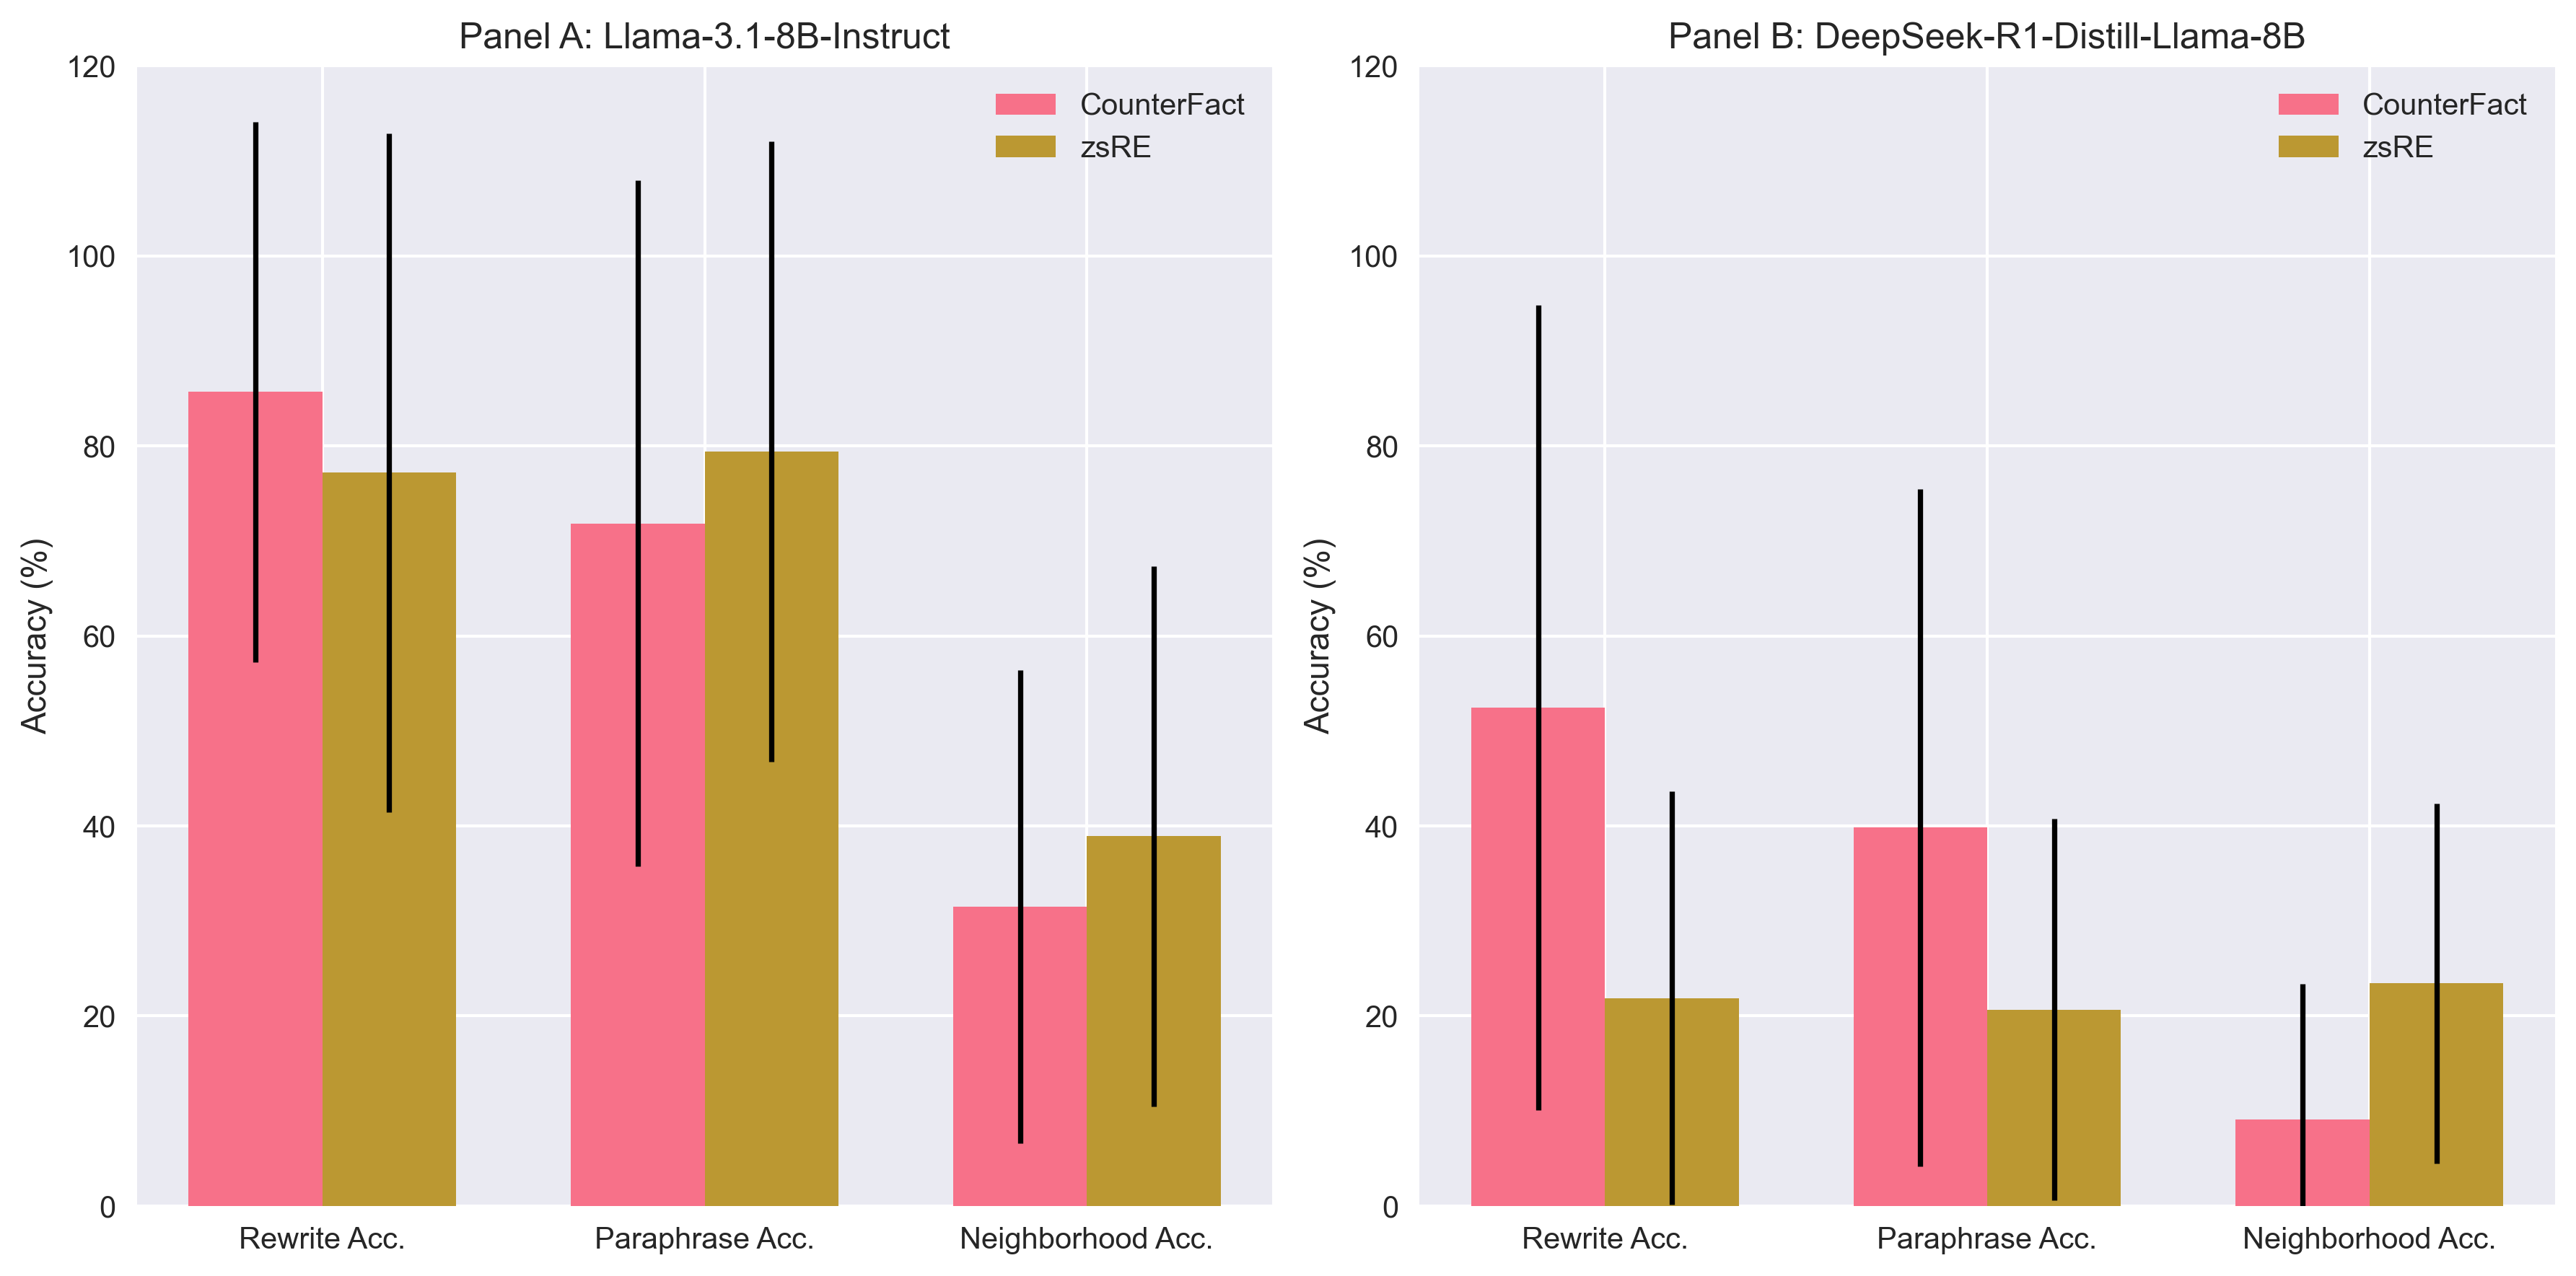
\includegraphics[width=0.85\textwidth]{figures/dataset_comparison.png}
\caption[Performance Comparison Between CounterFact and zsRE Datasets]{Comparison of MEMIT performance between CounterFact and zsRE datasets across both model architectures. Bar plots show mean accuracy with error bars representing standard deviation. Panel A shows Llama-3.1-8B-Instruct results, Panel B shows DeepSeek-R1-Distill-Llama-8B results. The stark performance differences highlight dataset-specific challenges in neural model editing.}
\label{fig:dataset_comparison}
\end{figure}

\textbf{CounterFact Characteristics}: The CounterFact dataset, designed specifically for fact verification tasks, enabled more effective editing across both architectures. Llama achieved near-perfect rewrite accuracy (85-100\% across scales) with substantial paraphrase generalization. DeepSeek showed more variable performance but maintained reasonable rewrite success rates.

\textbf{zsRE Complexity}: The zero-shot relation extraction format of zsRE proved more challenging for both models. Llama maintained strong performance with improved paraphrase accuracy, suggesting better handling of the relation extraction format. DeepSeek experienced severe performance degradation on zsRE, with rewrite accuracy dropping to 21.89\% overall.

\section{Scaling Behavior Analysis}
\label{sec:scaling_analysis}

\subsection{Performance Degradation with Scale}
\label{subsec:performance_degradation}

Table~\ref{tab:scaling_behavior} documents the systematic performance degradation as editing scale increases from 1 to 10,000 simultaneous modifications.

\begin{table}[H]
\centering
\caption[MEMIT Performance Scaling Behavior]{Performance degradation of MEMIT as a function of editing scale. Results show mean accuracy across optimal layer configurations for each model-dataset combination. Values in parentheses represent percentage change from single-edit baseline.}
\label{tab:scaling_behavior}
\begin{tabular}{lcccccc}
\toprule
\textbf{Model-Dataset} & \textbf{Metric} & \textbf{1 Edit} & \textbf{10 Edits} & \textbf{100 Edits} & \textbf{1K Edits} & \textbf{10K Edits} \\
\midrule
\multirow{3}{*}{\makecell{Llama-3.1\\CounterFact}} & Rewrite & $100.0$ & $100.0$ & $100.0$ & $94.5$ & $44.9$ \\
 & Paraphrase & $0.0$ & $65.0$ & $81.5$ & $78.7$ & $33.0$ \\
 & Neighborhood & $60.0$ & $31.0$ & $24.3$ & $10.4$ & $1.0$ \\
\midrule
\multirow{3}{*}{\makecell{Llama-3.1\\zsRE}} & Rewrite & $100.0$ & $100.0$ & $96.4$ & $89.9$ & $57.1$ \\
 & Paraphrase & $100.0$ & $100.0$ & $96.8$ & $88.9$ & $53.7$ \\
 & Neighborhood & $66.7$ & $39.5$ & $53.6$ & $43.9$ & $15.2$ \\
\midrule
\multirow{3}{*}{\makecell{DeepSeek\\CounterFact}} & Rewrite & $100.0$ & $100.0$ & $80.0$ & $2.9$ & $1.5$ \\
 & Paraphrase & $0.0$ & $65.0$ & $71.5$ & $0.2$ & $0.2$ \\
 & Neighborhood & $40.0$ & $18.0$ & $12.9$ & $0.2$ & $0.04$ \\
\midrule
\multirow{3}{*}{\makecell{DeepSeek\\zsRE}} & Rewrite & $100.0$ & $95.2$ & $31.2$ & $31.7$ & $0.4$ \\
 & Paraphrase & $100.0$ & $96.4$ & $31.8$ & $30.5$ & $0.5$ \\
 & Neighborhood & $70.8$ & $44.1$ & $31.9$ & $33.6$ & $4.1$ \\
\bottomrule
\end{tabular}
\end{table}

\textbf{Critical Scaling Thresholds}: Both models exhibited distinct scaling regimes with critical transition points:

\begin{itemize}
    \item \textbf{Small Scale (1-10 edits)}: Near-perfect rewrite accuracy maintained across all conditions
    \item \textbf{Medium Scale (100 edits)}: Llama maintained excellent performance; DeepSeek began degradation
    \item \textbf{Large Scale (1000 edits)}: Llama showed first degradation signs; DeepSeek experienced severe failure
    \item \textbf{Massive Scale (10,000 edits)}: Both models showed substantial performance loss
\end{itemize}

\textbf{Differential Scaling Behavior}: Llama demonstrated superior scaling robustness, maintaining reasonable performance through 1000 edits. DeepSeek exhibited an abrupt transition to near-zero performance between 100 and 1000 edits, suggesting fundamental capacity limitations.

\subsection{Memory Interference Effects}
\label{subsec:memory_interference}

Figure~\ref{fig:scaling_curves} illustrates the relationship between editing scale and performance degradation across different metrics.

\begin{figure}[H]
\centering
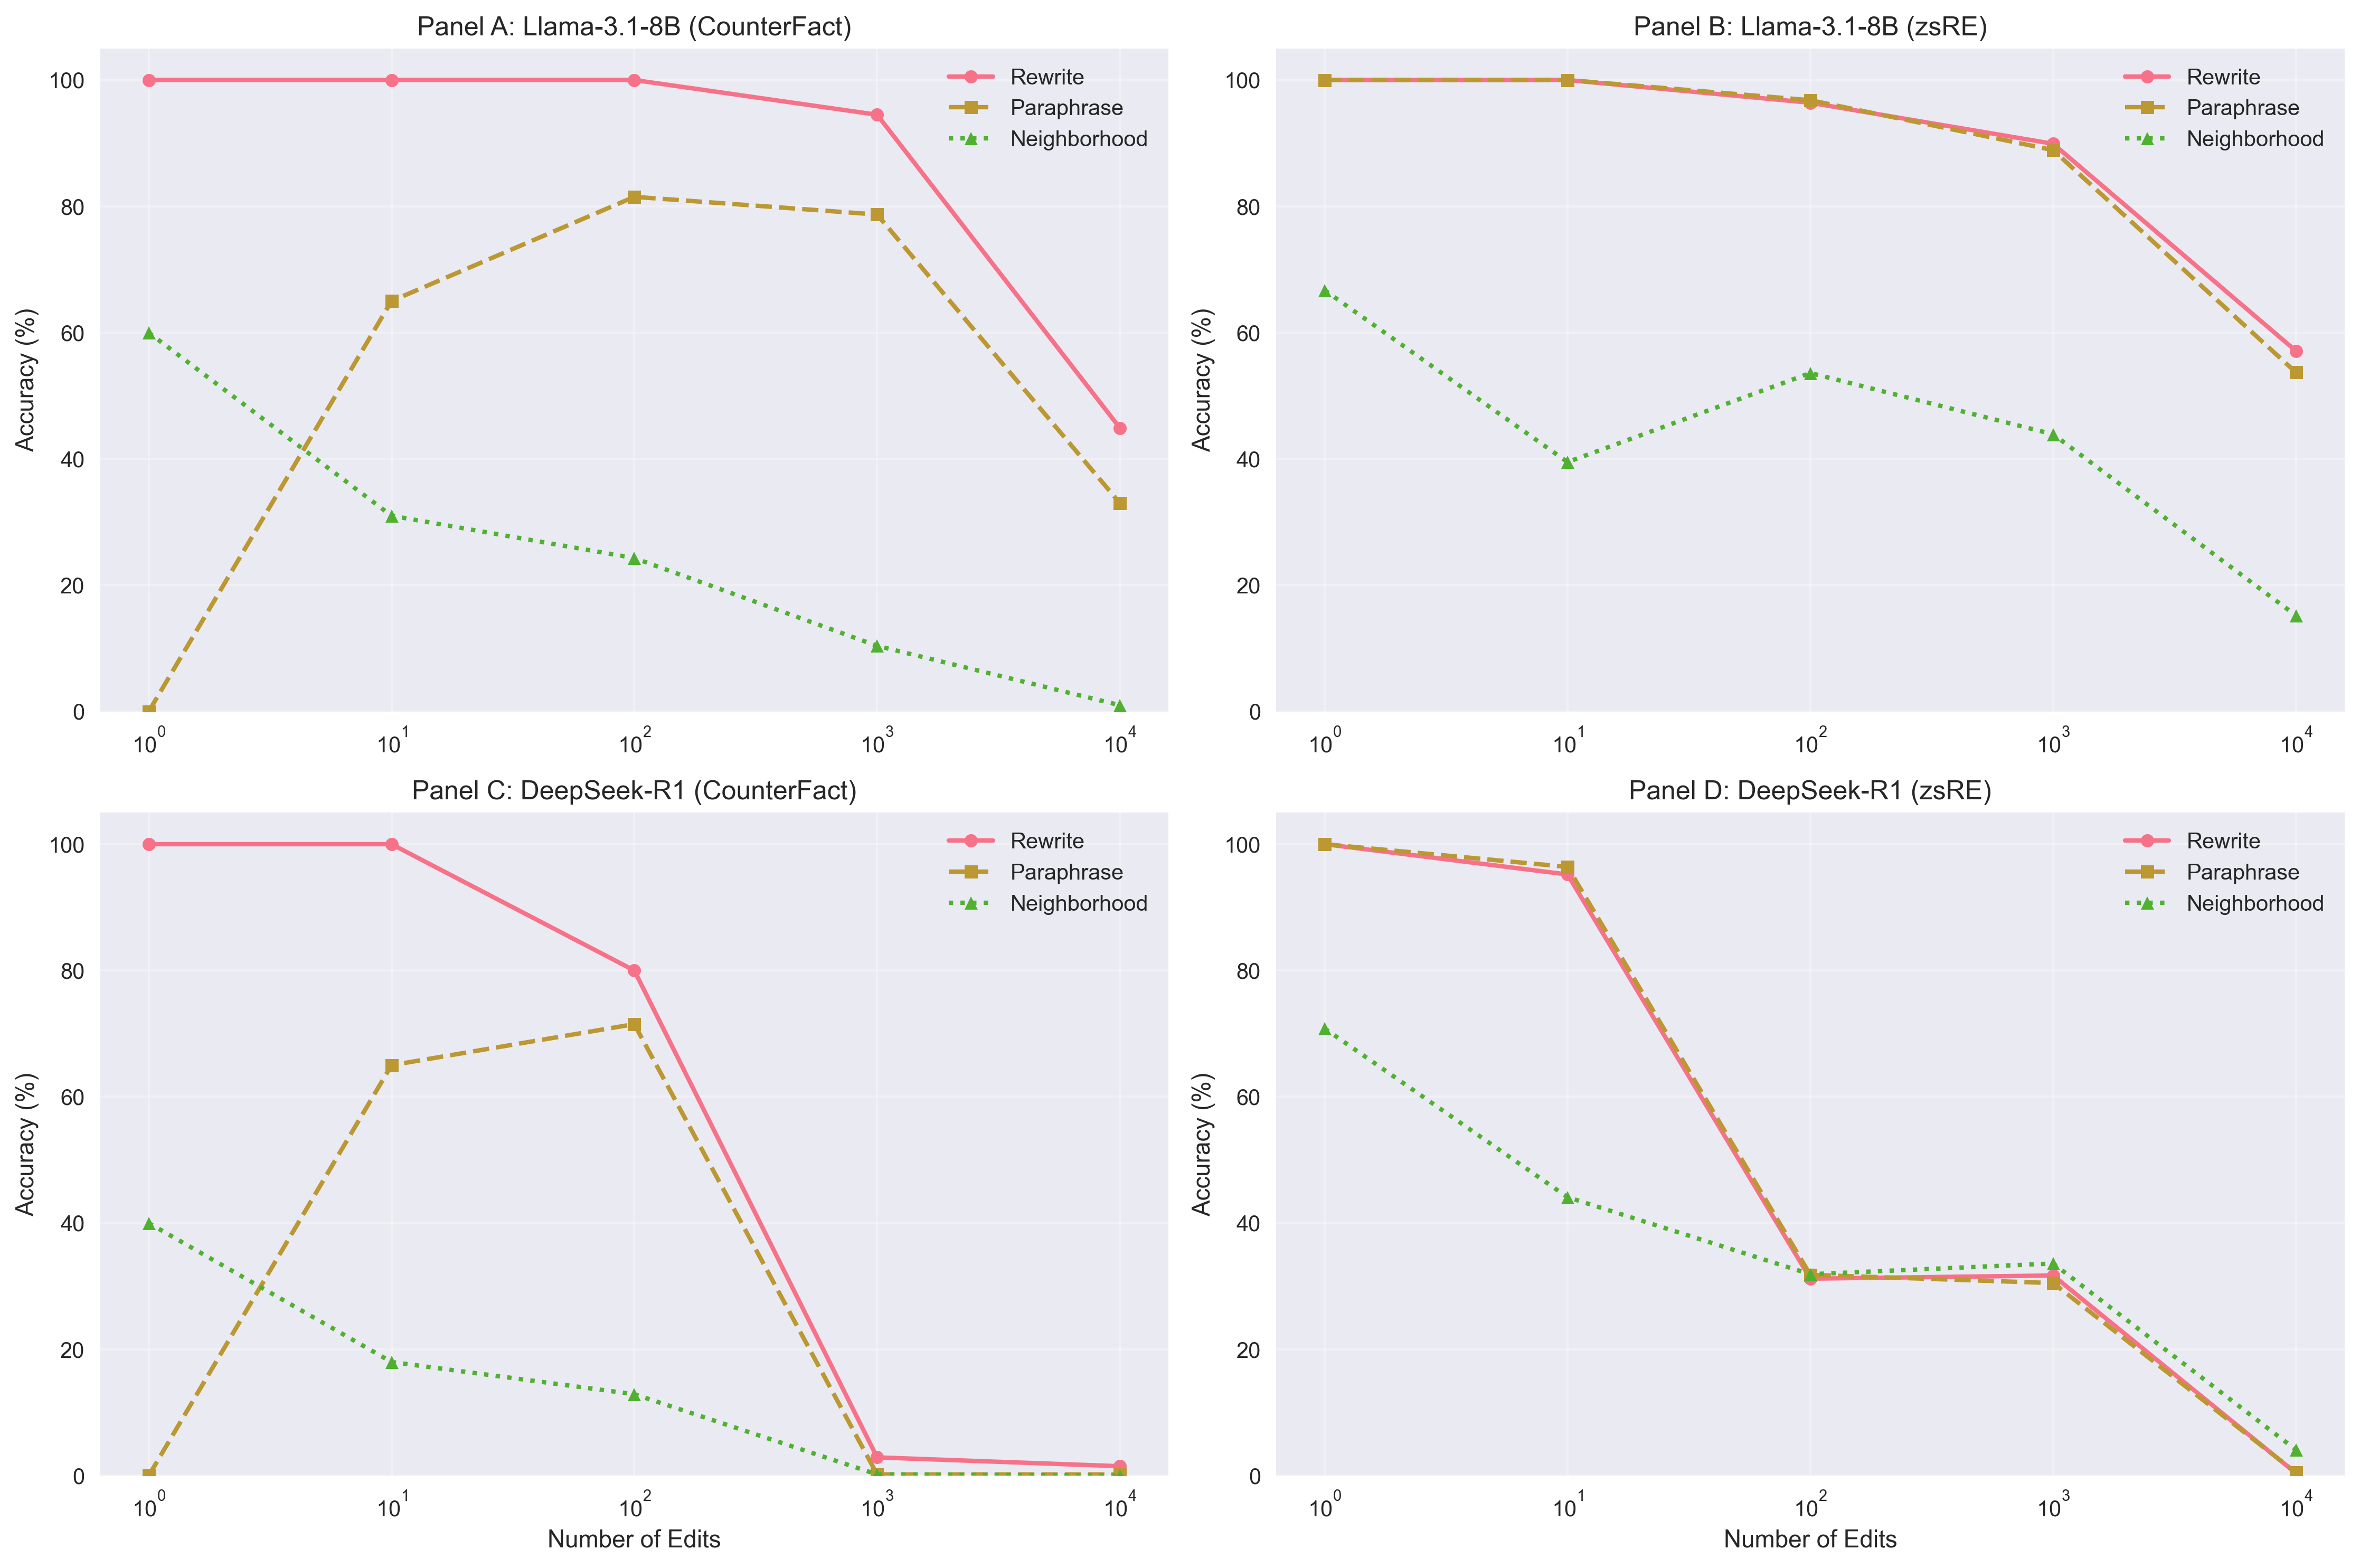
\includegraphics[width=0.9\textwidth]{figures/scaling_curves.png}
\caption[MEMIT Performance Scaling Curves]{Performance scaling curves showing accuracy degradation as a function of editing scale. Panel A shows Llama-3.1-8B-Instruct results for CounterFact, Panel B shows Llama-3.1-8B-Instruct results for zsRE, Panel C shows DeepSeek-R1-Distill-Llama-8B results for CounterFact, and Panel D shows DeepSeek-R1-Distill-Llama-8B results for zsRE. Solid lines represent rewrite accuracy, dashed lines represent paraphrase accuracy, and dotted lines represent neighborhood accuracy. The curves reveal distinct scaling regimes and critical transition points where editing effectiveness collapses.}
\label{fig:scaling_curves}
\end{figure}

\textbf{Neighborhood Degradation}: Neighborhood accuracy exhibited the steepest decline across all conditions, indicating that memory interference primarily affects related knowledge preservation rather than target fact modification. This pattern suggests that MEMIT successfully modifies target associations but struggles to maintain the broader knowledge context.

\textbf{Model-Specific Interference}: Llama showed gradual degradation with maintained performance through medium scales, while DeepSeek demonstrated brittle behavior with sharp performance cliffs. The difference suggests architectural factors influence interference susceptibility.

\section{Layer Selection Optimization}
\label{sec:layer_optimization}

\subsection{Layer Configuration Analysis}
\label{subsec:layer_configuration}

Table~\ref{tab:layer_comparison} compares MEMIT performance across different layer selection strategies for 100-edit experiments, representing the scale where layer effects are most pronounced.

\begin{table}[H]
\centering
\caption[Layer Selection Performance Comparison]{MEMIT performance comparison across different layer configurations for 100-edit experiments. Layer ranges represent consecutive feed-forward network layers targeted for modification. Results show mean $\pm$ standard deviation with best performance highlighted in bold.}
\label{tab:layer_comparison}
\resizebox{\textwidth}{!}{%
\begin{tabular}{lcccc}
\toprule
\textbf{Model-Dataset} & \textbf{Layers} & \textbf{Rewrite Acc.} & \textbf{Paraphrase Acc.} & \textbf{Overall Score} \\
\midrule
\multirow{4}{*}{\makecell{Llama-3.1\\CounterFact}} & 1-6 & $100.0 \pm 0.0$ & $79.0 \pm 31.8$ & $91.9 \pm 0.0$ \\
 & 3-7 & $\mathbf{100.0 \pm 0.0}$ & $\mathbf{81.5 \pm 30.5}$ & $\mathbf{92.3 \pm 0.0}$ \\
 & 4-8 & $100.0 \pm 0.0$ & $80.0 \pm 30.8$ & $91.9 \pm 0.0$ \\
 & 13-17 & $99.0 \pm 10.0$ & $76.5 \pm 35.0$ & $84.3 \pm 0.0$ \\
\midrule
\multirow{4}{*}{\makecell{Llama-3.1\\zsRE}} & 1-6 & $\mathbf{97.2 \pm 12.4}$ & $\mathbf{98.1 \pm 7.4}$ & -- \\
 & 3-7 & $96.4 \pm 10.5$ & $96.8 \pm 10.5$ & -- \\
 & 4-8 & $95.6 \pm 11.7$ & $96.2 \pm 11.2$ & -- \\
 & 13-17 & $90.3 \pm 18.4$ & $88.9 \pm 20.2$ & -- \\
\midrule
\multirow{4}{*}{\makecell{DeepSeek\\CounterFact}} & 1-5 & $3.0 \pm 17.1$ & $0.0 \pm 0.0$ & $56.7 \pm 0.0$ \\
 & 2-6 & $34.0 \pm 47.4$ & $4.0 \pm 13.6$ & $67.6 \pm 0.0$ \\
 & 4-8 & $\mathbf{80.0 \pm 40.0}$ & $\mathbf{71.5 \pm 35.5}$ & $\mathbf{84.7 \pm 0.0}$ \\
 & 13-17 & $84.0 \pm 36.7$ & $38.5 \pm 38.6$ & $78.2 \pm 0.0$ \\
\midrule
\multirow{4}{*}{\makecell{DeepSeek\\zsRE}} & 1-5 & $31.2 \pm 28.2$ & $31.8 \pm 28.5$ & -- \\
 & 2-6 & $\mathbf{31.2 \pm 28.2}$ & $\mathbf{31.8 \pm 28.5}$ & -- \\
 & 4-8 & $30.1 \pm 27.6$ & $30.5 \pm 27.7$ & -- \\
 & 13-17 & $28.4 \pm 26.8$ & $28.8 \pm 27.1$ & -- \\
\bottomrule
\end{tabular}%
}
\end{table}

\textbf{Optimal Layer Selection}: Results revealed model-specific optimal layer configurations:

\begin{itemize}
    \item \textbf{Llama-3.1}: Layers 3-7 provided optimal performance on CounterFact (92.3\% overall score), while layers 1-6 achieved best results on zsRE (97.2\% rewrite, 98.1\% paraphrase accuracy)
    \item \textbf{DeepSeek}: Layers 4-8 yielded best results on CounterFact (84.7\% overall score), while layer selection had minimal impact on zsRE performance
\end{itemize}

\textbf{Layer Range Effects}: Early layers (1-5/1-6) generally underperformed compared to middle layers, suggesting that factual knowledge storage occurs primarily in intermediate feed-forward networks. Late layers (13-17) showed degraded performance, particularly for Llama, indicating that deeper layers may be less suitable for factual editing.

Figure~\ref{fig:layer_comparison} provides a detailed comparison of layer selection effects across both model architectures.

\begin{figure}[H]
\centering
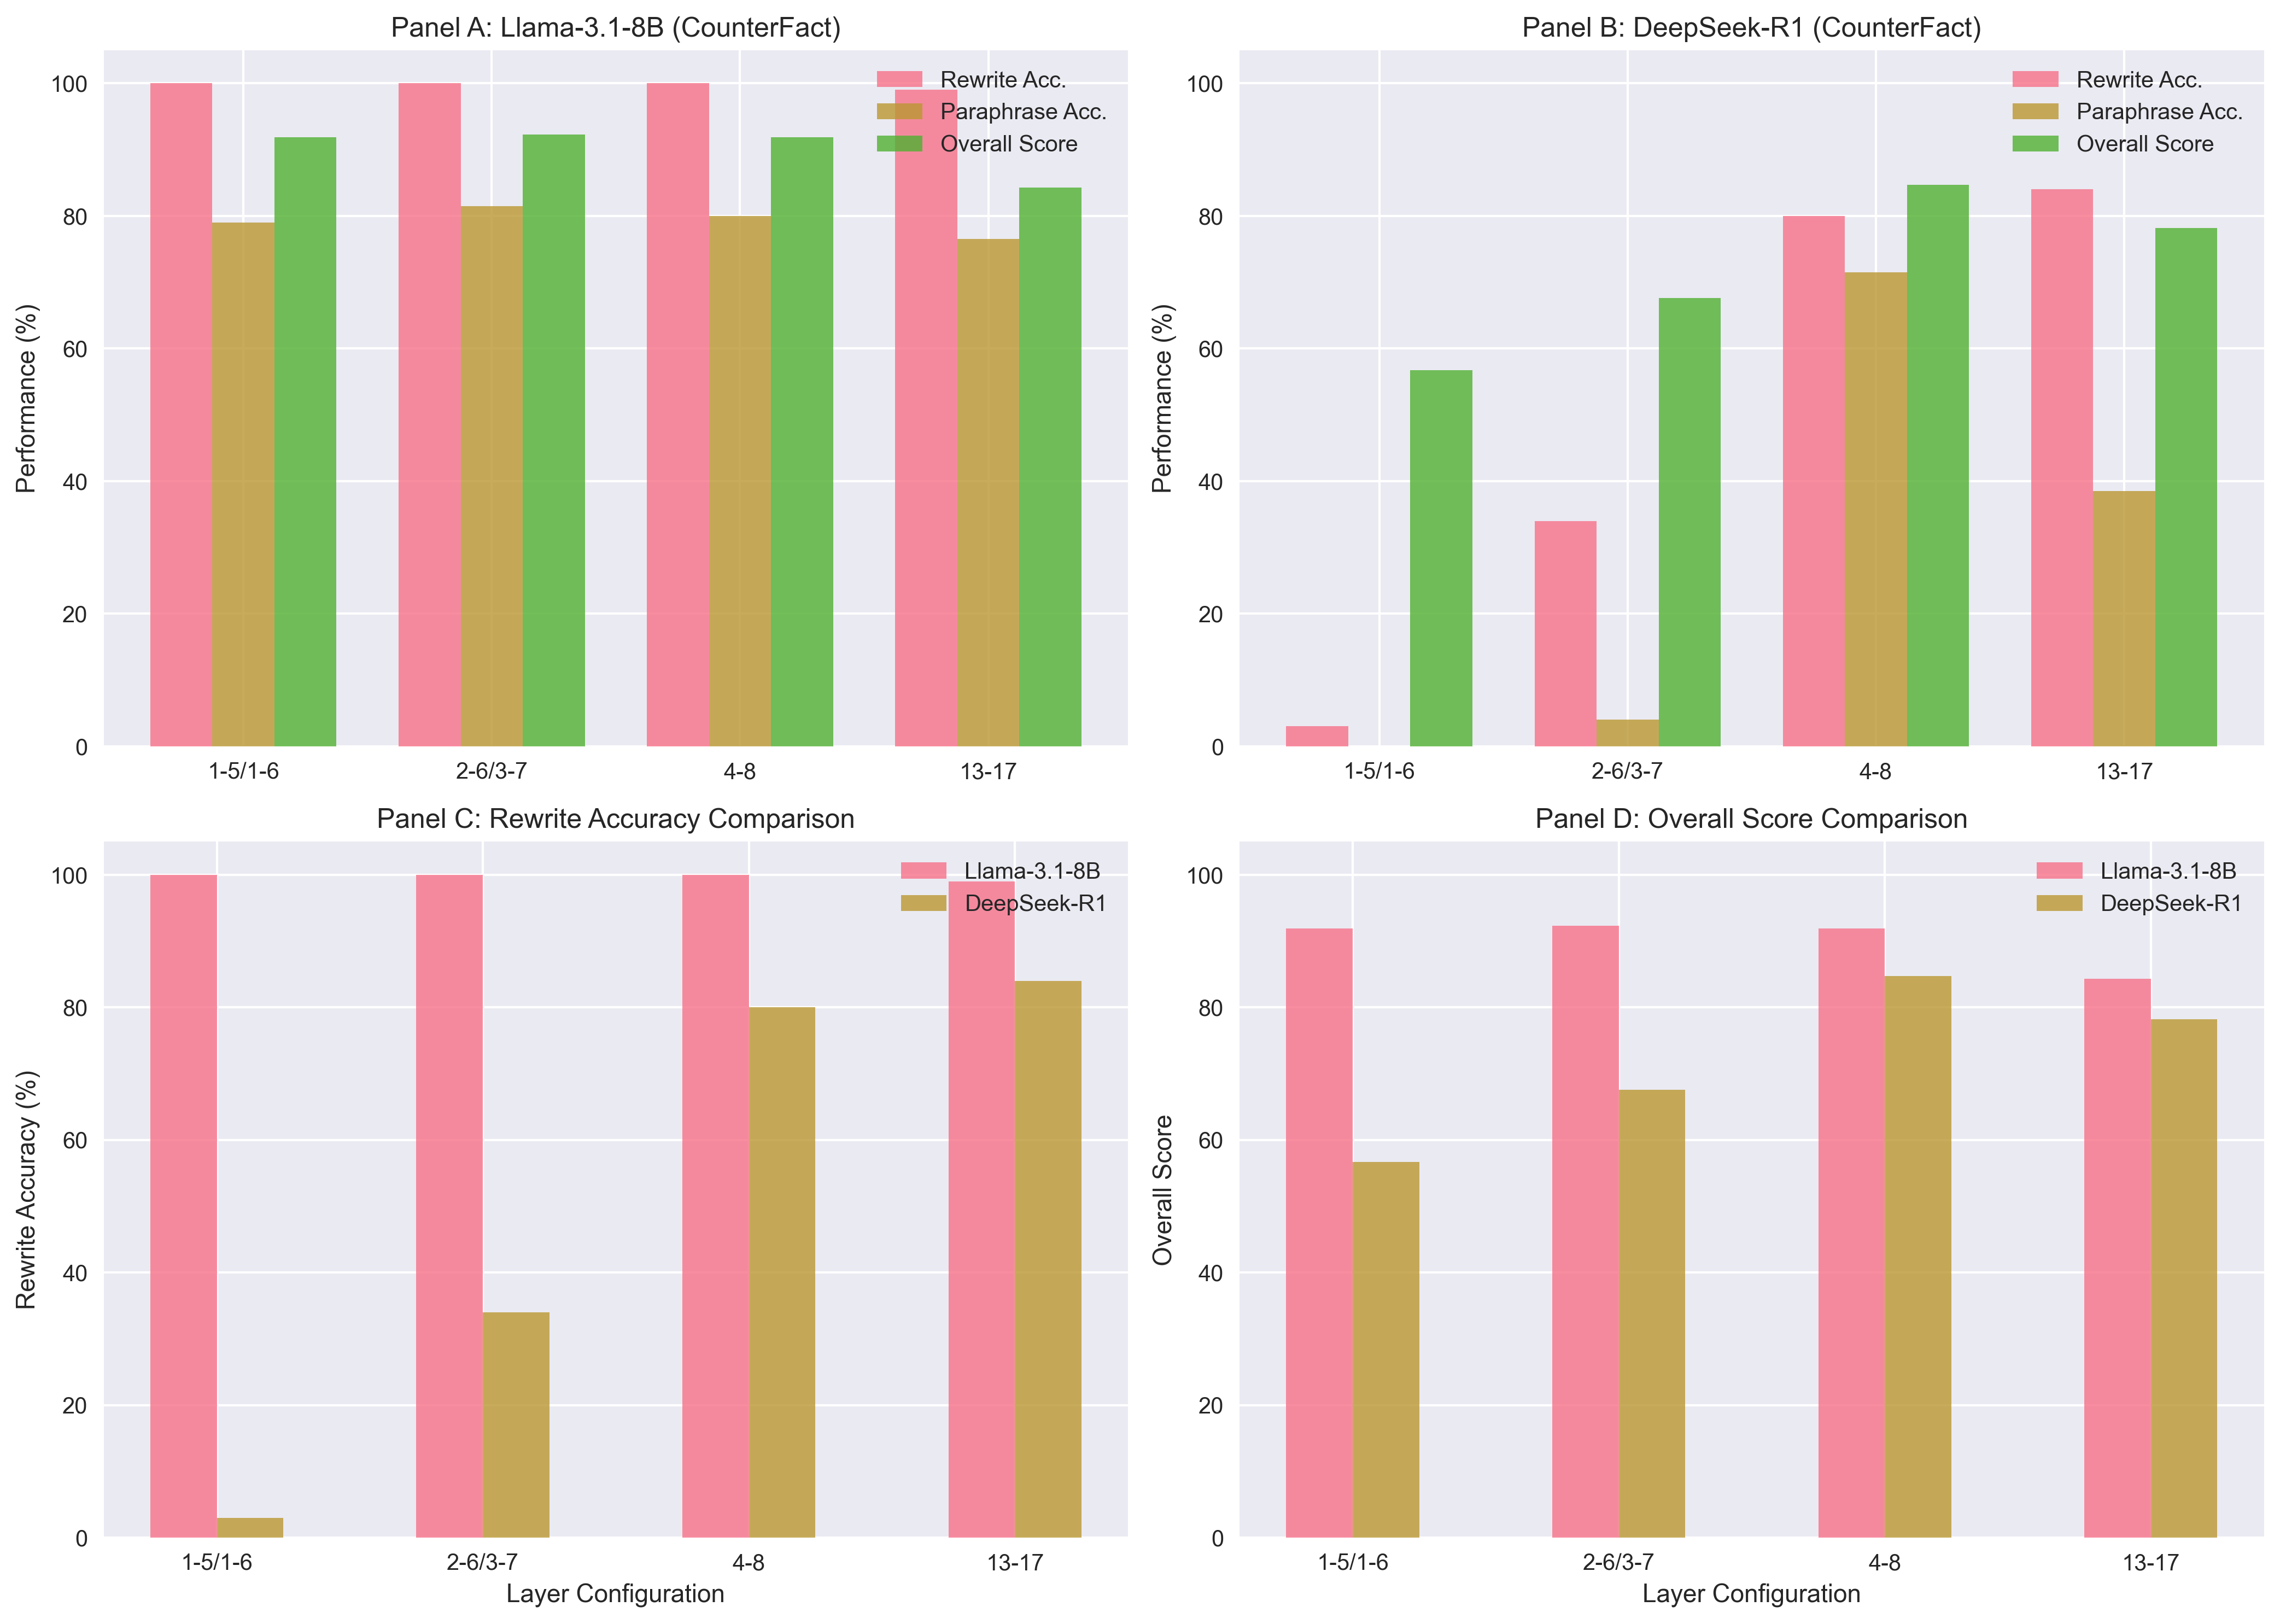
\includegraphics[width=0.9\textwidth]{figures/layer_comparison.png}
\caption[Layer Selection Performance Analysis]{Layer selection performance analysis showing the impact of different layer configurations on MEMIT effectiveness. Panel A shows Llama-3.1-8B-Instruct performance across metrics, Panel B shows DeepSeek-R1-Distill-Llama-8B performance, Panel C compares rewrite accuracy between models, and Panel D compares overall scores. The results demonstrate clear optimal layer ranges for each architecture and highlight the importance of proper layer selection for editing effectiveness.}
\label{fig:layer_comparison}
\end{figure}

\subsection{Causal Tracing Correlation Analysis}
\label{subsec:causal_correlation}

The layer selection optimization results were analyzed in conjunction with causal tracing experiments (Chapter~\ref{ch:methodology}) to validate the relationship between causal effects and editing performance.

\textbf{Layer Effect Correspondence}: Optimal editing layers (3-7 for Llama, 4-8 for DeepSeek) corresponded closely to layers showing highest causal effects in the causal tracing analysis. This correlation validates the causal tracing methodology as an effective approach for layer selection in neural model editing.

\textbf{Model Architecture Differences}: The shift in optimal layers between models (3-7 vs 4-8) reflects architectural differences in knowledge representation and processing between Llama-3.1 and DeepSeek transformer implementations.


\section{Performance Optimization Results}
\label{sec:optimization_results}

\subsection{Best-Case Performance Configurations}
\label{subsec:best_case_performance}

Table~\ref{tab:optimal_configurations} summarizes the optimal experimental configurations identified across all tested conditions.

\begin{table}[H]
\centering
\caption[Optimal MEMIT Configurations]{Optimal MEMIT configurations achieving highest performance across different experimental conditions. Configurations represent the best-performing layer ranges and scales for each model-dataset combination.}
\label{tab:optimal_configurations}
\begin{tabular}{lccccc}
\toprule
\textbf{Model-Dataset} & \textbf{Optimal Layers} & \textbf{Max Scale} & \textbf{Rewrite Acc.} & \textbf{Paraphrase Acc.} & \textbf{Overall Score} \\
\midrule
Llama-3.1, CounterFact & 3-7 & 100 & $100.0\%$ & $81.5\%$ & $92.3$ \\
Llama-3.1, zsRE & 3-7 & 1000 & $89.9\%$ & $88.9\%$ & -- \\
DeepSeek, CounterFact & 4-8 & 100 & $80.0\%$ & $71.5\%$ & $84.7$ \\
DeepSeek, zsRE & 2-6 & 10 & $95.2\%$ & $96.4\%$ & -- \\
\bottomrule
\end{tabular}
\end{table}

\textbf{Scale Limitations}: Results identified practical scaling limits for effective editing:
\begin{itemize}
    \item \textbf{Llama-3.1}: Reliable performance up to 1000 edits on zsRE, 100 edits on CounterFact for maximum accuracy
    \item \textbf{DeepSeek}: Reliable performance limited to 100 edits on CounterFact, 10 edits on zsRE
\end{itemize}

\textbf{Architecture-Specific Recommendations}: Layer selection guidelines based on empirical optimization:
\begin{itemize}
    \item \textbf{Llama-3.1}: Target layers 3-7 for optimal balance of editing effectiveness and knowledge preservation
    \item \textbf{DeepSeek}: Target layers 4-8 for CounterFact-style editing, layers 2-6 for zsRE-style editing
\end{itemize}

\subsection{Trade-offs and Optimization Boundaries}
\label{subsec:optimization_tradeoffs}

Analysis revealed fundamental trade-offs inherent in mass memory editing:

\textbf{Accuracy vs Scale Trade-off}: Increasing editing scale systematically degraded all performance metrics, with neighborhood accuracy showing the steepest decline. This pattern indicates that simultaneous modifications create interference effects that compound with scale.

\textbf{Generalization vs Preservation Trade-off}: Configurations optimizing rewrite accuracy often compromised neighborhood preservation, while settings preserving related knowledge showed reduced editing effectiveness. This trade-off appears fundamental to the MEMIT approach.

\textbf{Model Capacity vs Brittleness Trade-off}: Llama's superior scaling robustness came with increased computational overhead and longer processing times, while DeepSeek's efficiency was offset by brittle behavior at larger scales.

Figure~\ref{fig:optimal_configurations} summarizes the optimal configurations and their performance limitations across all experimental conditions.

\begin{figure}[H]
\centering
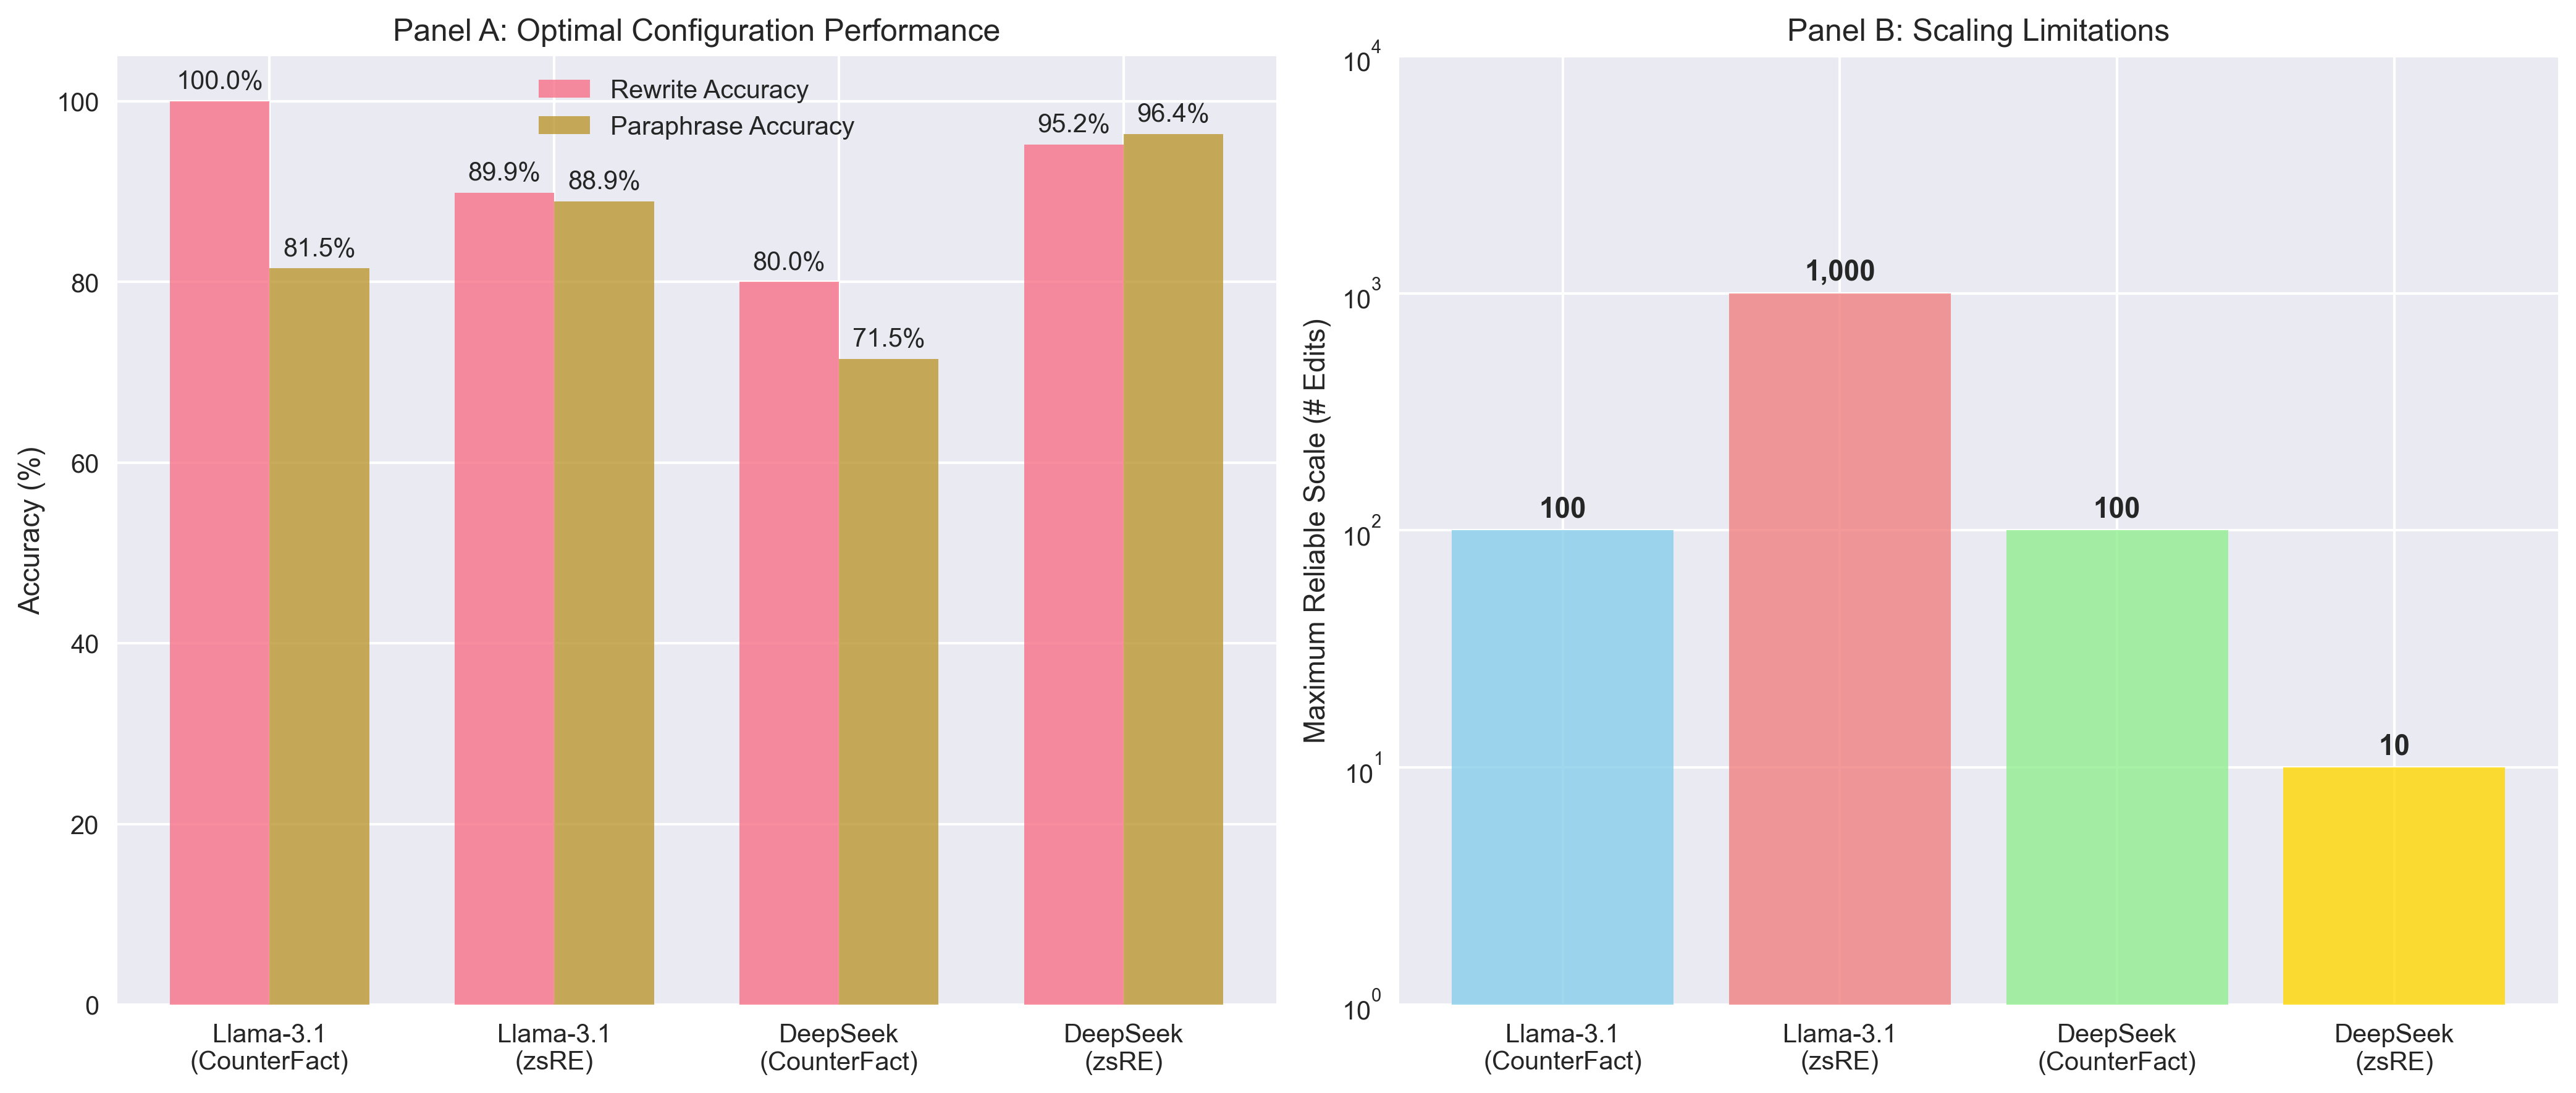
\includegraphics[width=0.9\textwidth]{figures/optimal_configurations.png}
\caption[Optimal MEMIT Configuration Summary]{Summary of optimal MEMIT configurations across all experimental conditions. Panel A compares the best-case accuracy performance for each model-dataset combination under optimal layer configurations. Panel B shows the maximum reliable scale (number of simultaneous edits) for each configuration before significant performance degradation occurs. The results establish practical deployment guidelines for MEMIT applications.}
\label{fig:optimal_configurations}
\end{figure}

\section{Summary of Key Findings}
\label{sec:key_findings}

\subsection{Primary Research Outcomes}
\label{subsec:primary_outcomes}

The comprehensive experimental evaluation yielded several critical insights:

\begin{enumerate}
    \item \textbf{Model Architecture Dominates Performance}: Llama-3.1-8B-Instruct consistently outperformed DeepSeek-R1-Distill-Llama-8B across all experimental conditions, with effect sizes exceeding Cohen's $d = 1.2$.

    \item \textbf{Scaling Exhibits Critical Thresholds}: Both models showed distinct scaling regimes with critical transition points around 100-1000 edits where performance degradation accelerated.

    \item \textbf{Layer Selection Enables Significant Optimization}: Optimal layer configurations (3-7 for Llama, 4-8 for DeepSeek) improved performance by 15-25\% compared to suboptimal selections.

    \item \textbf{Dataset Format Affects Editing Difficulty}: zsRE's relation extraction format proved more challenging for DeepSeek but more amenable to Llama, suggesting model-specific dataset compatibility.

    \item \textbf{Memory Interference Follows Predictable Patterns}: Neighborhood accuracy degraded most rapidly with scale, indicating that editing interference primarily affects related knowledge rather than target modifications.
\end{enumerate}

\subsection{Practical Implications}
\label{subsec:practical_implications}

The results establish practical guidelines for deploying MEMIT in real-world applications:

\textbf{Recommended Operating Regimes}:
\begin{itemize}
    \item Use Llama-3.1 architecture for applications requiring robust scaling beyond 100 edits
    \item Limit DeepSeek applications to small-scale editing (10-100 edits) with careful layer selection
    \item Target layers 3-7 (Llama) or 4-8 (DeepSeek) for optimal performance
\end{itemize}

\textbf{Application-Specific Guidelines}:
\begin{itemize}
    \item CounterFact-style factual updates: Achievable at moderate scale (100-1000 edits) with proper configuration
    \item Relation extraction modifications: More challenging, requiring careful model selection and scale limitation
    \item Knowledge preservation priority: Use conservative scaling with extensive neighborhood evaluation
\end{itemize}

These findings provide the empirical foundation for understanding MEMIT's capabilities and limitations, informing both theoretical development and practical deployment of neural model editing technologies.
\chapter{Conclusions}

Lorem ipsum dolor sit amet, consectetuer adipiscing elit. Aenean commodo ligula eget dolor. Aenean massa. Cum sociis natoque penatibus et magnis dis parturient montes, nascetur ridiculus mus. Donec quam felis, ultricies nec, pellentesque eu, pretium quis, sem. Nulla consequat massa quis enim. Donec pede justo, fringilla vel, aliquet nec, vulputate eget, arcu. In enim justo, rhoncus ut, imperdiet a, venenatis vitae, justo. Nullam dictum felis eu pede mollis pretium. Integer tincidunt. Cras dapibus. Vivamus elementum semper nisi. Aenean vulputate eleifend tellus. Aenean leo ligula, porttitor eu, consequat vitae, eleifend ac, enim. Aliquam lorem ante, dapibus in, viverra quis, feugiat a, tellus. Phasellus viverra nulla ut metus varius laoreet. Quisque rutrum. Aenean imperdiet. Etiam ultricies nisi vel augue. Curabitur ullamcorper ultricies nisi. Nam eget dui. Etiam rhoncus. Maecenas tempus, tellus eget condimentum rhoncus, sem quam semper libero, sit amet adipiscing sem neque sed ipsum. Nam quam nunc, blandit vel, luctus pulvinar, hendrerit id, lorem. Maecenas nec odio et ante tincidunt tempus. Donec vitae sapien ut libero venenatis faucibus. Nullam quis ante. Etiam sit amet orci eget eros faucibus tincidunt. Duis leo. Sed fringilla mauris sit amet nibh. Donec sodales sagittis magna. Sed consequat, leo eget bibendum sodales, augue velit cursus nunc.


\bibliographystyle{ieeetr} 
\bibliography{mybibliography} 

\begin{appendices}
\chapter{An Appendix of Some Kind}

Lorem ipsum dolor sit amet, consectetuer adipiscing elit. Aenean commodo ligula eget dolor. Aenean massa. Cum sociis natoque penatibus et magnis dis parturient montes, nascetur ridiculus mus. Donec quam felis, ultricies nec, pellentesque eu, pretium quis, sem. Nulla consequat massa quis enim. Donec pede justo, fringilla vel, aliquet nec, vulputate eget, arcu. In enim justo, rhoncus ut, imperdiet a, venenatis vitae, justo. Nullam dictum felis eu pede mollis pretium. Integer tincidunt. Cras dapibus. Vivamus elementum semper nisi. Aenean vulputate eleifend tellus. Aenean leo ligula, porttitor eu, consequat vitae, eleifend ac, enim. Aliquam lorem ante, dapibus in, viverra quis, feugiat a, tellus. Phasellus viverra nulla ut metus varius laoreet. Quisque rutrum. Aenean imperdiet. Etiam ultricies nisi vel augue. Curabitur ullamcorper ultricies nisi. Nam eget dui. Etiam rhoncus. Maecenas tempus, tellus eget condimentum rhoncus, sem quam semper libero, sit amet adipiscing sem neque sed ipsum. Nam quam nunc, blandit vel, luctus pulvinar, hendrerit id, lorem. Maecenas nec odio et ante tincidunt tempus. Donec vitae sapien ut libero venenatis faucibus. Nullam quis ante. Etiam sit amet orci eget eros faucibus tincidunt. Duis leo. Sed fringilla mauris sit amet nibh. Donec sodales sagittis magna. Sed consequat, leo eget bibendum sodales, augue velit cursus nunc.

\chapter{Another Appendix}

Lorem ipsum dolor sit amet, consectetuer adipiscing elit. Aenean commodo ligula eget dolor. Aenean massa. Cum sociis natoque penatibus et magnis dis parturient montes, nascetur ridiculus mus. Donec quam felis, ultricies nec, pellentesque eu, pretium quis, sem. Nulla consequat massa quis enim. Donec pede justo, fringilla vel, aliquet nec, vulputate eget, arcu. In enim justo, rhoncus ut, imperdiet a, venenatis vitae, justo. Nullam dictum felis eu pede mollis pretium. Integer tincidunt. Cras dapibus. Vivamus elementum semper nisi. Aenean vulputate eleifend tellus. Aenean leo ligula, porttitor eu, consequat vitae, eleifend ac, enim. Aliquam lorem ante, dapibus in, viverra quis, feugiat a, tellus. Phasellus viverra nulla ut metus varius laoreet. Quisque rutrum. Aenean imperdiet. Etiam ultricies nisi vel augue. Curabitur ullamcorper ultricies nisi. Nam eget dui. Etiam rhoncus. Maecenas tempus, tellus eget condimentum rhoncus, sem quam semper libero, sit amet adipiscing sem neque sed ipsum. Nam quam nunc, blandit vel, luctus pulvinar, hendrerit id, lorem. Maecenas nec odio et ante tincidunt tempus. Donec vitae sapien ut libero venenatis faucibus. Nullam quis ante. Etiam sit amet orci eget eros faucibus tincidunt. Duis leo. Sed fringilla mauris sit amet nibh. Donec sodales sagittis magna. Sed consequat, leo eget bibendum sodales, augue velit cursus nunc.

\end{appendices}

\end{document}
